\chapter{Verification and Completion}\label{chap:verification}
\chapintro{This chapter is based on results published in~\cite{LohmannKLR_2007_wsfm}.}
%%%%%%%%%%%%%%%%%%%%%%%%%%%%%%%%%%%%%%%%%%%%%%%%%%%%%%%%%%%%%%%%%%%%%%%%%%%%%


\lettrine[findent=.2em,lines=2,nindent=0pt]{I}{n} the previous two chapters, we investigated the correctness of services in isolation; that is, services embedded in arbitrary environments. With the notion of controllability and behavioral constraints, we could reason about the correctness of \emph{one} service with respect to \emph{any} possible service composition. In this chapter, we go one step further and study the correctness of a \emph{concrete} composition of \emph{several} services.

As in the previous chapters, we focus on the behavior of service compositions and employ compatibility as correctness criterion. For this reason, we do not consider other aspects of composing services, such as wiring (\ie, addressing and syntactical issues), instance lifecycles (\ie, how new instances are created, who triggers instantiations, and how many ``copies'' of each service are needed), or nonfunctional properties (\eg, an agreement on encryption, policies, or quality of service). 

In the literature~\cite{Peltz_2003_ieee,DijkmanD_2004_ijcis}, two viewpoints on a service composition are distinguished: \emph{service orchestrations} and \emph{service choreographies}. They are typically considered to be complementary paradigms, whereas other authors (\eg,~\cite{PapazoglouTDL_2007_ieee}) criticize a too strict distinction. We shall come back to this discussion in \autoref{chap:realizability}.

A service orchestration (cf.~\autoref{fig:orchestration}) takes the \emph{viewpoint of a single participant}. It focuses on this \emph{orchestrator} and abstracts from the internal behavior of other participants. The service orchestrator only considers the ports to the other participants rather than their concrete behavior or their interaction between third parties. Service orchestrations are well-suited to describe a business process whose activities are executed by other services. For the execution of service orchestrations, the language \acronym{WS-BPEL}~\cite{standard_bpel} emerged as a de-facto standard. A \acronym{WS-BPEL} process specifies how other services are invoked and includes all information that are required to execute it on an engine.

A service choreography (cf.~\autoref{fig:choreography}) takes the \emph{global viewpoint} on a service composition and does not focus on individual participants. From a modeling perspective, choreographies can be used as a bottom-up approach (called \emph{interconnected models}) or as a top-down approach (called \emph{interaction models}).

%%%%%%%%%%%%%%%%%%%%%%%%%%%%%%%%%%%%%%%%%%%%%%%%%%%%%%%%%%%%%%%%%%%%%%%%%%%%%%
\begin{figure}[t!]
\centering
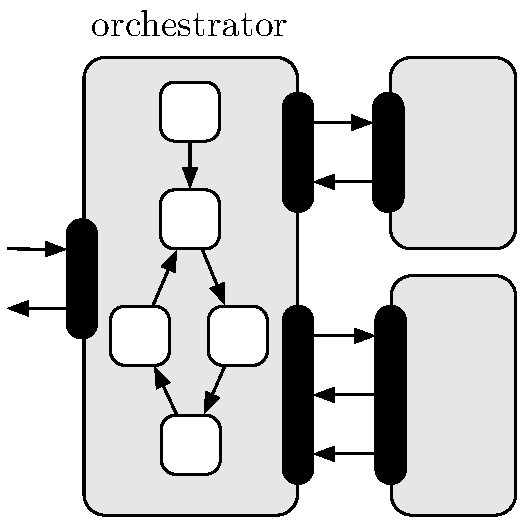
\includegraphics[scale=0.45]{verification/orchestrator}\caption{Service orchestration.}\label{fig:orchestration}
%\end{figure}
%\begin{figure}
%\centering
%\vspace{1em}
\subfigure[interconnected model\label{fig:interconnected}]{\hspace{14em}}\hfill
\subfigure[interaction model\label{fig:interaction}]{\hspace{14em}}
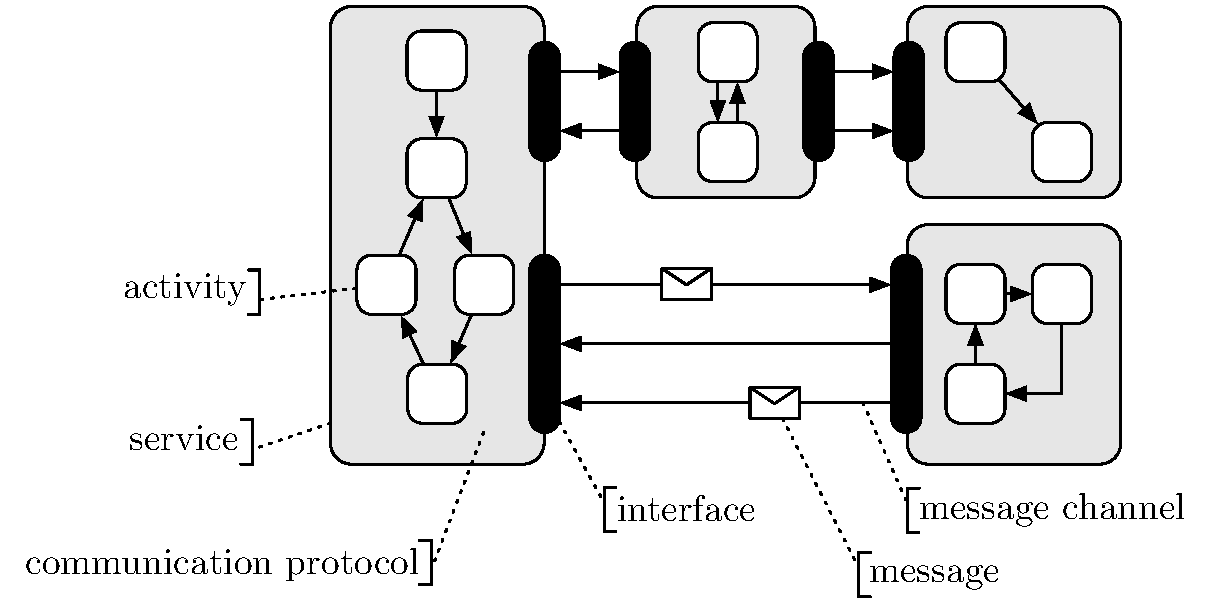
\includegraphics[width=\textwidth]{verification/overview}
\caption{Service choreography.}\label{fig:choreography}
\end{figure}
%%%%%%%%%%%%%%%%%%%%%%%%%%%%%%%%%%%%%%%%%%%%%%%%%%%%%%%%%%%%%%%%%%%%%%%%%%%%%%

In the paradigm of interconnected models (cf.\ \autoref{fig:interconnected}), several local service models are merged into a service choreography; that is, services are composed. This can be seen as bottom-up approach, because the global behavior of the choreography is determined by wiring already specified services. It is the classical scenario of \acronym{SOC} (also called \emph{programming in the large}~\cite{DeRemerK_1976_tse}) facilitating the design of large systems by composing smaller building blocks. The language \bpelchor~\cite{DeckerKLW_2007_icws} has been introduced to specify global interactions by reusing \acronym{WS-BPEL} processes.

\enlargethispage*{\baselineskip}

In contrast, the top-down approach, used by the interaction model paradigm (cf. \autoref{fig:interaction}), starts with a specification of the desired global behavior of a service composition which is yet to be realized. This interaction model is then projected to the participating services and refined toward execution. Interaction modeling aims at early design stages of service compositions and is typically used to model novel interorganizational business processes rather than already established compositions. We shall investigate interaction models in \autoref{chap:realizability}.

\medskip

In this chapter, we investigate the correctness of interconnected models (\ie, service compositions) specified in the language \bpelchor. To this end, we continue as follows. The next section briefly introduces the languages \acronym{WS-BPEL} and \bpelchor. In \autoref{sec:Translation}, we give a formalization of these languages in terms service automata. To facilitate this translation, we employ Petri nets as intermediate formalism, because they offer a compact representation of service automata. \Autoref{sec:Analysis} is devoted to the compatibility analysis of \bpelchor\ choreographies. Experimental results show that the verification techniques scale to choreographies with up to a thousand participants. In \autoref{sec:ver:syn}, the completion of partially specified choreographies is studied. By applying results from previous chapters, we can automatically synthesize stub processes for incomplete choreographies. Finally, \autoref{sec:ver:related} presents related work and \autoref{sec:ver:conclusion} concludes the chapter.





%%%%%%%%%%%%%%%%%%%%%%%%%%%%%%%%%%%%%%%%%%%%%%%%%%%%%%%%%%%%%%%%%%%%%%%%%%%%%%%
\section[WS-BPEL and BPEL4Chor]{WS-BPEL and BPEL{\footnotesize 4}Chor}




%%%%%%%%%%%%%%%%%%%%%%%%%%%%%%%%%%%%%%%%%%%%%%%%%%%%%%%%%%%%%%%%%%%%%%%%%%%%%%
\subsection*{WS-BPEL}

The \emph{Web Services Business Process Execution Language} (\acronym{WS-BPEL}) \cite{standard_bpel}, is a domain-specific language for describing the behavior of business processes based on Web services. This makes \acronym{WS-BPEL} a language for the \emph{programming in the large} paradigm~\cite{DeRemerK_1976_tse}. Its focus is\,---\,unlike modifying variable values in classical programming languages such as C or Java\,---\,the message exchange and interaction with other Web services. Advanced concepts such as instantiation, complex exception handling, and compensation of long running transactions are further features which are needed to implement business processes. These features are first-class citizens in \acronym{WS-BPEL}. In this section, we shall only give a brief overview of those concepts of the language which are relevant in this thesis. The interested reader is referred to detailed introductions \cite{wsbpelprimer,wsbook,AlonsoCKM_2003}.

For the specification of a business process, \acronym{WS-BPEL} provides \emph{activities} and distinguishes between basic and structured activities. A~basic activity can exchange messages with other services (\bpel{invoke}, \bpel{receive}, \bpel{reply}), manipulate and validate data, wait for a period of time or just do nothing (\bpel{empty}), signal faults, invoke a compensation handler, or end the entire process instance.

A structured activity defines a causal execution order on basic activities and can be nested in another structured activity itself. The structured activities include sequential execution (\bpel{sequence}), parallel execution (\bpel{flow}), data-dependent branching (\bpel{if}), timeout- or message-dependent branching (\bpel{pick}), and repeated execution (\bpel{repeatUntil}, \bpel{while}, and \bpel{forEach}). Within activities executed in parallel, the execution order can further be controlled by the usage of \emph{control links}. A control link has a source and a target activity. With Boolean conditions, the splitting and joining behavior can be controlled. If a target activity has to be skipped due to negative evaluation of its join condition, all outgoing control links are set to false, which may cause other activities to be skipped, which is called \emph{dead-path elimination}~\cite{LeymannR_1999_dpe}.

In addition, the structured activity \bpel{scope} links fault, compensation, termination, and event handling to an activity. The \bpel{process} is the outmost scope of the described business process. A \bpel{faultHandler} provides methods to react to faults, which may occur during execution, whereas a \bpel{compensationHandler} can be used to reverse the effects of successfully executed scopes. With the help of an \bpel{eventHandler}, external message events and specified timeouts can be handled. The forced termination of running scopes is controlled by a \bpel{terminationHandler}.

\acronym{WS-BPEL} supports two kind of process specifications. On the one hand, an \emph{executable process} contains all information required to be deployed and executed on a \acronym{WS-BPEL} engine. On the other hand, \acronym{WS-BPEL} further allows to leave parts of the process unspecified. In such \emph{abstract processes}, a placeholder such as an \bpel{opaqueActivity} can be used which is later replaced by concrete activities or branching conditions. An abstract process implicitly specifies a set of executable completions.

Although \acronym{WS-BPEL} is intended as exchange and documentation format, it is based on \acronym{XML} and provides no graphical representation. This makes visualization and specification cumbersome. Hence, every vendor of \acronym{WS-BPEL} development tools introduced proprietary graphical notations. In this thesis, we employ \acronym{BPMN}~\cite{standard_bpmn} as graphical representation. \Autoref{fig:verfication:bpmn} provides an overview of the \acronym{BPMN} constructs used in this thesis. The level of abstraction of \acronym{BPMN} is similar to that of service automata. In particular, the order in which messages are sent and received, the initial state, and final states can be easily derived from a \acronym{BPMN} diagram. In addition, the upcoming \acronym{BPMN} standard~\cite{standard_bpmn2} provides a basic mapping between \acronym{BPMN} and \acronym{WS-BPEL}.

%%%%%%%%%%%%%%%%%%%%%%%%%%%%%%%%%%%%%%%%%%%%%%%%%%%%%%%%%%%%%%%%%%%%%%%%%%%%%%
\begin{figure}[tb]
\centering
{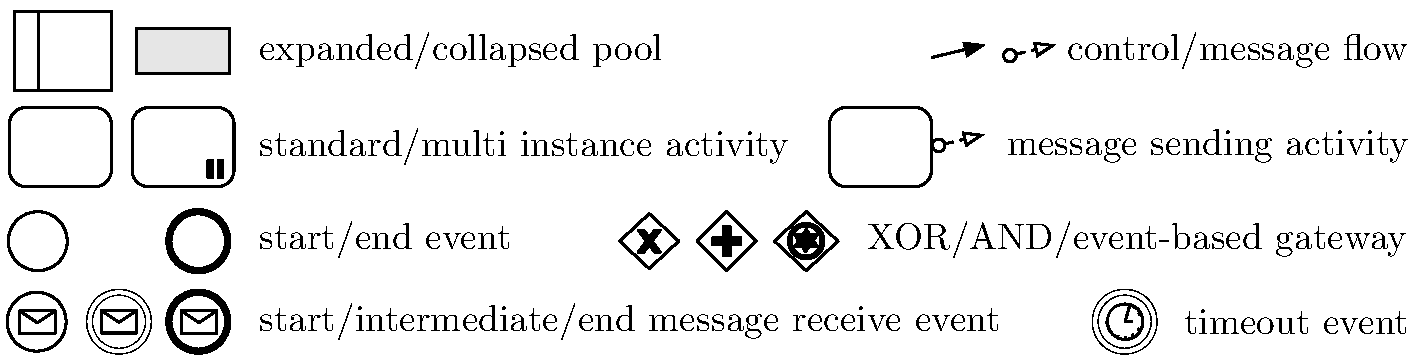
\includegraphics[scale=0.45]{verification/bpmn}}
\caption{\acronym{BPMN} in a nutshell.}\label{fig:verfication:bpmn}
\end{figure}
%%%%%%%%%%%%%%%%%%%%%%%%%%%%%%%%%%%%%%%%%%%%%%%%%%%%%%%%%%%%%%%%%%%%%%%%%%%%%%

%%%%%%%%%%%%%%%%%%%%%%%%%%%%%%%%%%%%%%%%%%%%%%%%%%%%%%%%%%%%%%%%%%%%%%%%%%%%%%
\begin{figure}[tb]
\centering
\subfigure[abstract WS-BPEL process\label{fig:verification:traveler:bpel}]{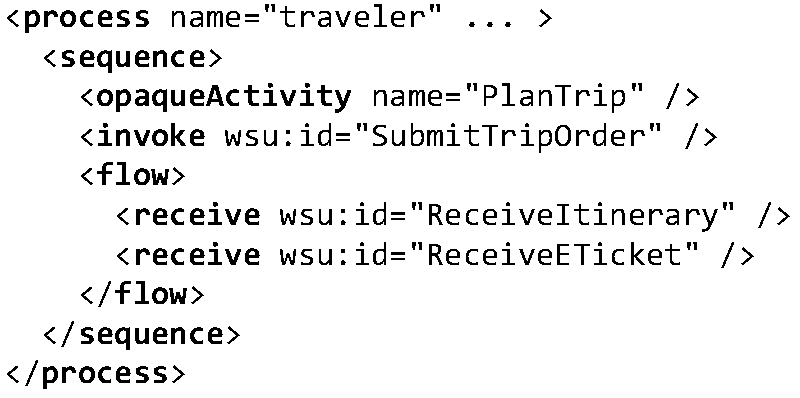
\includegraphics[scale=0.45]{verification/traveler_bpel}}
\subfigure[BPMN visualization\label{fig:verification:traveler:bpmn}]{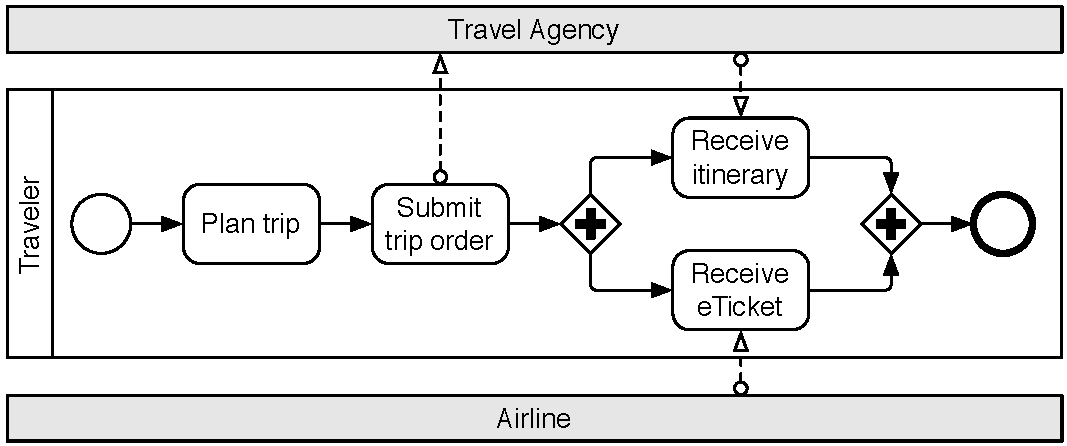
\includegraphics[scale=0.45]{verification/traveler_bpmn}}
\caption{Traveler service.}\label{fig:verification:traveler}
\end{figure}
%%%%%%%%%%%%%%%%%%%%%%%%%%%%%%%%%%%%%%%%%%%%%%%%%%%%%%%%%%%%%%%%%%%%%%%%%%%%%%



\paragraph{Example.}

In this chapter, we investigate a choreography modeling a ticket booking scenario taken from~\cite{DeckerKLW_2007_icws}. It consists of several participants: a \emph{traveler} who sends a trip order (\ie, a request to book a particular trip) to a \emph{travel agency}, which in turn queries several \emph{airline services} for prices and chooses the cheapest offer. Finally, the traveler receives an itinerary from the travel agency and an e-ticket from the chosen airline. \Autoref{fig:verification:traveler:bpel} depicts the traveler's perspective modeled as an abstract \acronym{WS-BPEL} process. In this service orchestration, only the behavior of the traveler is explicitly specified inside an expanded pool, whereas the behavior of the travel agency and the airline services is left unspecified. In \acronym{BPMN} notation, this is modeled by collapsed pools (depicted gray in \autoref{fig:verification:traveler:bpmn}).




%%%%%%%%%%%%%%%%%%%%%%%%%%%%%%%%%%%%%%%%%%%%%%%%%%%%%%%%%%%%%%%%%%%%%%%%%%%%%%
\subsection*{BPEL{\footnotesize 4}Chor}

%%%%%%%%%%%%%%%%%%%%%%%%%%%%%%%%%%%%%%%%%%%%%%%%%%%%%%%%%%%%%%%%%%%%%%%%%%%%%%
\begin{figure}[tb]
\centering
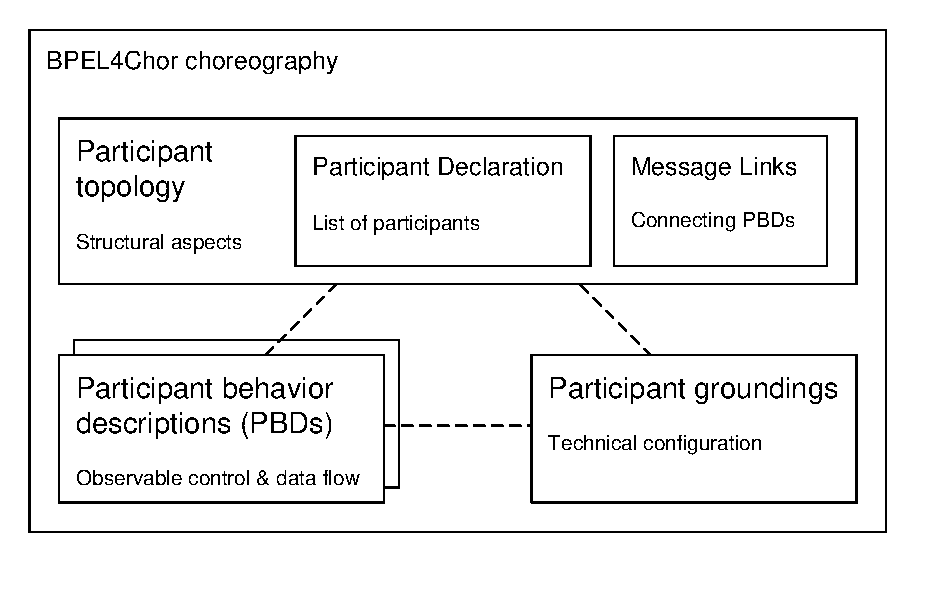
\includegraphics[width=0.7\textwidth]{verification/artifacttypes}
\caption{Artifacts of a \bpelchor{} choreography~\cite{DeckerKLW_2007_icws,DeckerKLW_2009_dke}.}\label{fig:artifacts}
\end{figure}
%%%%%%%%%%%%%%%%%%%%%%%%%%%%%%%%%%%%%%%%%%%%%%%%%%%%%%%%%%%%%%%%%%%%%%%%%%%%%%

%%%%%%%%%%%%%%%%%%%%%%%%%%%%%%%%%%%%%%%%%%%%%%%%%%%%%%%%%%%%%%%%%%%%%%%%%%%%%%
\begin{figure}[tb]
\centering
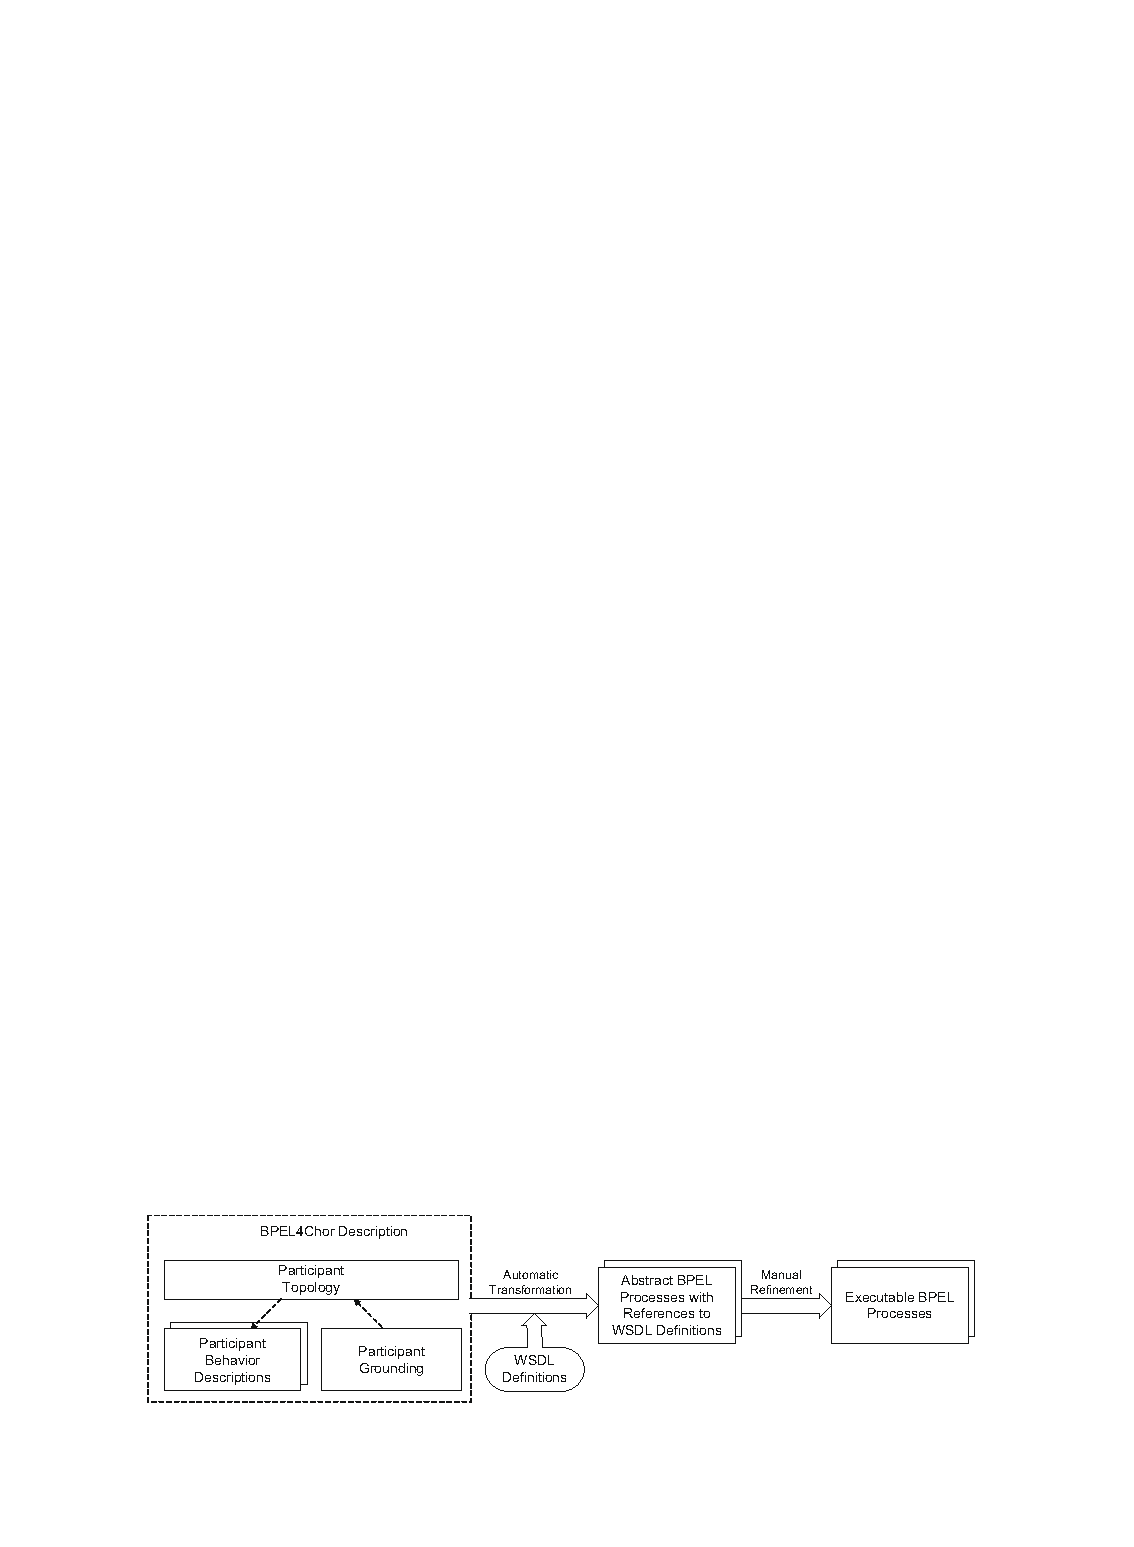
\includegraphics[width=\textwidth]{verification/translate}
\caption{Workflow from a \bpelchor{} choreography description to executable \acronym{WS-BPEL} processes~\cite{DeckerKLW_2009_dke}.}\label{fig:bpelchortrans}
\end{figure}
%%%%%%%%%%%%%%%%%%%%%%%%%%%%%%%%%%%%%%%%%%%%%%%%%%%%%%%%%%%%%%%%%%%%%%%%%%%%%%

Similar to the traveler service, the other participants' behavior can be specified using \acronym{WS-BPEL}. To describe the interaction of several \acronym{WS-BPEL} processes from a global perspective, \bpelchor{}~\cite{DeckerKLW_2007_icws} has been introduced as a choreography description language based on \acronym{WS-BPEL}. \bpelchor{} is not an execution language, but a means to specify all aspects which are required to execute several \acronym{WS-BPEL} processes as a choreography. This approach aims at reducing complexity by reusing services and execution infrastructure. A choreography described by \bpelchor{} consists of (1)~the \emph{participant topology}, (2) the \emph{participant behavior descriptions} (\acronym{PBD}s), and (3) the \emph{participant groundings} (cf.\ \autoref{fig:artifacts} and \cite{DeckerKLW_2007_icws,DeckerKLW_2009_dke}). The participant topology lists all participants taking part in the choreography and all message links connecting activities of different participants. \bpelchor{} allows for the specification of \emph{participant sets} to group several instances of a participant type. These sets can be (sequentially or parallely) traversed using \acronym{WS-BPEL}'s \bpel{forEach} activity. A \emph{message link} states that a message is sent from the source of the message link to its target. A \bpelchor\ choreography always describes the behavior of all participants. Thus, a \emph{closed world} is assumed.

Every participant has a certain type. For each participant type, a participant behavior description defined in \acronym{WS-BPEL} is given. In this description, port types and operations are omitted and thus the dependency on interface specifications such as \acronym{WSDL}~\cite{standard_wsdl} is removed; that is, the \acronym{PBD}s are abstract \acronym{WS-BPEL} processes. To execute the choreography, every target of a message link has to be grounded to a \acronym{WSDL} operation so that the other participants can use the offered operation. This grounding is done after the choreography design itself, which enables choreography specification reuse. As \acronym{WS-BPEL} is used to specify the behavior of every participant, the development of executable \acronym{WS-BPEL} processes implementing this behavior can be done by using the \acronym{PBD} of a participant as a basis and adding missing details. \citet{ReimannKDL_2008_tr0807} elaborate this process. \Autoref{fig:bpelchortrans} diagrams the overall workflow from a \bpelchor{} choreography to executable \acronym{WS-BPEL} processes. Even though other languages can be used to provide implementations of local behavior, using \acronym{WS-BPEL} is a seamless choice using \bpelchor{}.

\enlargethispage*{2\baselineskip}

\paragraph{Example.}

\Autoref{fig:broken} shows the complete ticket booking scenario from \cite{DeckerKLW_2007_icws}. It specifies the behavior of all participants; that is, all pools are expanded and there is no message exchange with any undefined participants. The multiple airline instances are modeled as follows. The airline pools are stacked and the ``request price'' activity is executed in a multiple instances activity modeling a parallel \bpel{forEach} activity. After receiving a quote from each of the airline instances, a choice is made. Activity ``order tickets'' sends a confirmation message to the selected instance. Finally, a timer event is used to terminate unchosen airline instances.

%%%%%%%%%%%%%%%%%%%%%%%%%%%%%%%%%%%%%%%%%%%%%%%%%%%%%%%%%%%%%%%%%%%%%%%%%%%%%%
\begin{figure}
\centering
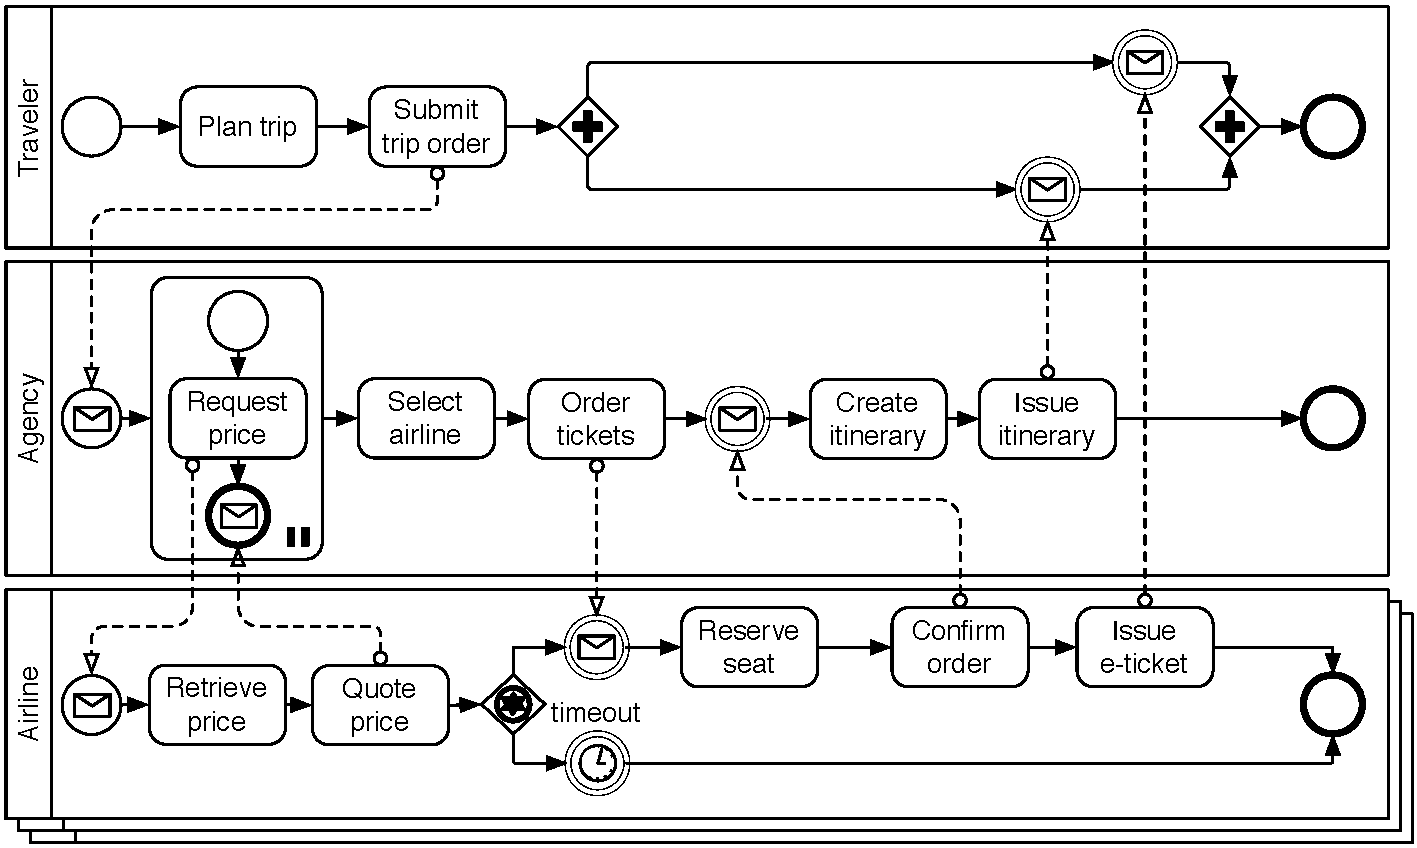
\includegraphics[scale=0.45]{verification/choreo}
\caption{Choreography of a ticket booking scenario, taken from~\cite{DeckerKLW_2007_icws}.}\label{fig:broken}
\end{figure}
%%%%%%%%%%%%%%%%%%%%%%%%%%%%%%%%%%%%%%%%%%%%%%%%%%%%%%%%%%%%%%%%%%%%%%%%%%%%%%





%%%%%%%%%%%%%%%%%%%%%%%%%%%%%%%%%%%%%%%%%%%%%%%%%%%%%%%%%%%%%%%%%%%%%%%%%%%%%%%
\section[Formalizing WS-BPEL and BPEL4Chor]{Formalizing WS-BPEL and BPEL{\footnotesize 4}Chor}
\label{sec:Translation}
%%%%%%%%%%%%%%%%%%%%%%%%%%%%%%%%%%%%%%%%%%%%%%%%%%%%%%%%%%%%%%%%%%%%%%%%%%%%%%%

The \acronym{WS-BPEL} language specification~\cite{standard_bpel} describes the operational semantics of \acronym{WS-BPEL} in natural language. This might be sufficient to understand \acronym{WS-BPEL}, but leaves room for ambiguities, contradictions, or unspecified behavior. A formalization~\cite{HinzSS_2005_bpm} of a predecessor specification~\cite{bpel4ws} revealed such unspecified situations which were resolved in the current specification. To \emph{formally} reason about \acronym{WS-BPEL} processes (\ie, to proof or to verify properties), \emph{formal semantics} are needed. Therefore, a lot of work has been conducted to give formal semantics for the behavior of \acronym{WS-BPEL} processes. The approaches cover many formalisms such as Petri nets, automata, abstract state machines, process algebras, and so on~\cite{BreugelK2006,LohmannVOSA_2009_ijbpim,LohmannVD_2008_topnoc}. A few  approaches are feature-complete and try to formalize every aspect of \acronym{WS-BPEL}. These approaches usually aim at a deeper understanding the language. Usually, however, only a subset of a language is formalized to investigate a certain aspect.

In the setting of this thesis, we focus on the \emph{behavior} of a \acronym{WS-BPEL} process. We abstract from other aspects such as time, instantiation, or data. In~\cite{Lohmann_2007_wsfm,Lohmann_2007_hubtr212}, we presented a translation from \acronym{WS-BPEL} to a class of Petri nets. Petri net-based formalisms have the advantage that they are closely related to automata, but can natively express concurrency which facilitates the specification of distributed systems. This make Petri nets an ideal intermediate formalism between \acronym{WS-BPEL} in which concurrency is very common and service automata, the basic formalism of this thesis.




%%%%%%%%%%%%%%%%%%%%%%%%%%%%%%%%%%%%%%%%%%%%%%%%%%%%%%%%%%%%%%%%%%%%%%%%%%%%%%
\subsection*{Petri nets}

\emph{Petri nets}~\cite{Reisig_1985,Murata_1989_pieee} are a formalism which was introduced to model and reason about distributed systems. Locality of the cause and effect of actions are realized consequently. This is reflected by the absence of a global notion of a state in favor of a distribution of resources throughout the system. In addition, Petri nets have a natural graphical representation, which was used as inspiration for later graphical notations such as \acronym{UML} activity diagrams or \acronym{BPMN}.

As already discussed in \autoref{chap:background:discussion}, the algorithm for controllability relies on global states and does not exploit concurrency. To this end, we use service automata as formal model in this thesis. However, Petri nets can be used to compactly represent larger service automata. At the same time, the ability to model distributed systems makes Petri nets a convenient intermediate formalism to translate industrial languages such as \acronym{WS-BPEL} into service automata. 

As Petri nets are not the main topic of this thesis, but just an intermediate formalism, we do not further discuss the specifics of the model, but continue with defining \emph{service nets}, a class of Petri nets, which is tailored to the needs of this chapter. The interested reader is referred to detailed introductions by~\citet{Reisig_1985}, \citet{Murata_1989_pieee}, and \citet{DeselR_1996_pn}.

%%%%%%%%%%%%%%%%%%%%%%%%%%%%%%%%%%%%%%%%%%%%%%%%%%%%%%%%%%%%%%%%%%%%%%%%%%%%%%
\begin{definition}{Service net}%
\label{def:servicenet}%
\nomenclature[N]{$N$}{a service net}%
A \emph{service net} is a tuple $N=[P,T,F,m_0,\Omega,\mathcal{P},\ell]$ such that
\begin{myitemize}
\item $P$ is a finite set of places,
\item $T$ is a finite set of transitions ($P\cap T=\emptyset$),
\item $F\subseteq (P\times T) \cup (T\times P)$ is a flow relation,
\item $m_0\in \Bags(P)$ is an initial marking,
\item $\Omega\subseteq \Bags(P)$ is a set of final markings,
\item $\mathcal{P}$ is an interface, and
\item $\ell: T\rightarrow (\E_\mathcal{P}\cup\{\tau\})$ a labeling function.
\end{myitemize}
\end{definition}
%%%%%%%%%%%%%%%%%%%%%%%%%%%%%%%%%%%%%%%%%%%%%%%%%%%%%%%%%%%%%%%%%%%%%%%%%%%%%%

A service net consists of a classical place/transition net $[P,T,F,m_0]$, a set of final markings, which model desired final states, an interface, and a labeling function that labels each transition with $\tau$ or an event that is derived from the interface.

%%%%%%%%%%%%%%%%%%%%%%%%%%%%%%%%%%%%%%%%%%%%%%%%%%%%%%%%%%%%%%%%%%%%%%%%%%%%%%
\begin{figure}
\centering
\subfigure[$N_1$\label{fig:verification:servicenet}]{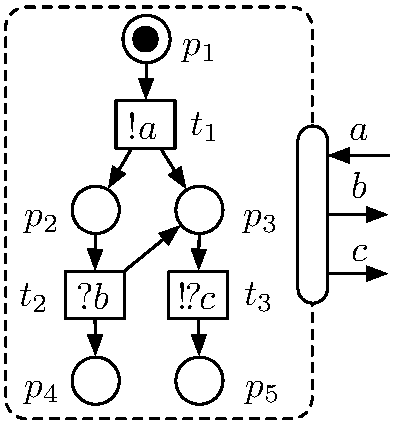
\includegraphics[scale=0.45]{verification/n1}}\hfill
\subfigure[$N_1$ after firing $t_{1}$\label{fig:verification:servicenet1}]{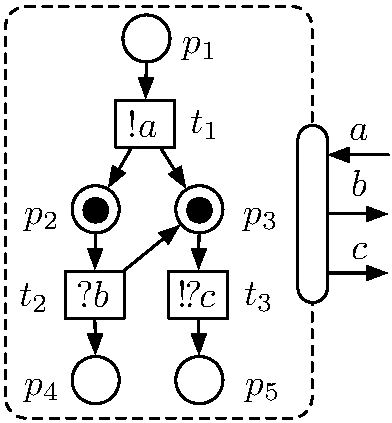
\includegraphics[scale=0.45]{verification/n1-1}}\hfill
\subfigure[$A_{N_1}$\label{fig:verification:servicenetsa}]{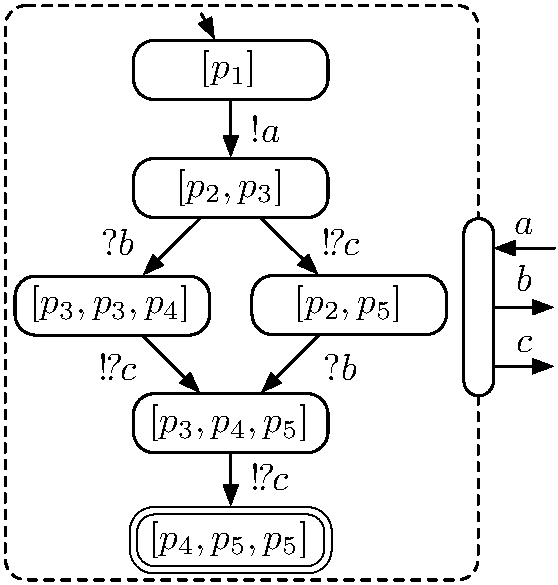
\includegraphics[scale=0.45]{verification/san1}}
\caption{A service net with $\Omega=\{\mset{p_{4},p_{5},p_{5}}\}$ (a) whose initial marking $m_{0}=[p_{1}]$ enables transition $t_{1}$. Firing~$t_{1}$ yields the marking $[p_{2},p_{3}]$~(b). The net can be translated into a service automaton~(c).}
\end{figure}
%%%%%%%%%%%%%%%%%%%%%%%%%%%%%%%%%%%%%%%%%%%%%%%%%%%%%%%%%%%%%%%%%%%%%%%%%%%%%%

We use the standard graphical notation for Petri nets and depict places by circles, transitions by rectangles, and the flow relation by directed arcs. A marking $m$ is represented by a distribution of $m(p)$ black dots (called ``tokens'') to each place $p$. Transition labels are written inside the transitions. Final markings have no graphical representation and are annotated to the net. We depict ports in the same way as for service automata. \Autoref{fig:verification:servicenet} shows an example.

\Autoref{def:servicenet} already suggests a close syntactical relationship to service automata. To give a mapping from a service net to a service automaton, we need to define the operational semantics of a service net; that is, we define a concept of states and state transitions. We do this by applying definitions known from place/transition nets.

%%%%%%%%%%%%%%%%%%%%%%%%%%%%%%%%%%%%%%%%%%%%%%%%%%%%%%%%%%%%%%%%%%%%%%%%%%%%%%
\begin{definition}{Firing rule}
\nomenclature[mtm]{$m \mathrel{[t\rangle}_N m'$}{firing transition $t$ in marking $m$ resulting marking $m'$}%
Let $N=[P,T,F,m_0,\Omega,\mathcal{P},\ell]$ be a service net. For a node $x\in P\cup T$, define the preset of $x$ as ${}^\bullet x:=\{y\mid [y,x]\in F\}$ and the postset of $x$ as $x^\bullet:=\{y\mid [x,y]\in F\}$.

A transition $t$ is \define{enabled} at marking $m\in\Bags(P)$ iff $m(p)>0$ holds for all places $p \in {}^\bullet x$. An enabled transition $t$ can \define{fire} in $m$, denoted $m \mathrel{[t\rangle}_N m'$, yielding the successor marking $m'$ with\vspace{-0.5em}
$$m'(p):=\begin{cases}
m(p)-1,&\text{iff $p\in {}^\bullet t \setminus t^\bullet$,}\\
m(p)+1,&\text{iff $p\in t^\bullet \setminus {}^\bullet t$,}\\
m(p),&\text{otherwise.}\end{cases}$$\vspace{-1em}
\end{definition}
%%%%%%%%%%%%%%%%%%%%%%%%%%%%%%%%%%%%%%%%%%%%%%%%%%%%%%%%%%%%%%%%%%%%%%%%%%%%%%

In the net of \autoref{fig:verification:servicenet}, transition $t_{1}$ is enabled in the initial marking. Firing $t_{1}$ yields a successor marking depicted in \autoref{fig:verification:servicenet1}. Now we can use markings of a service net as states of a service automaton. Likewise, the labeling of the service net's transitions can be used to derive a labeled transition relation.

%%%%%%%%%%%%%%%%%%%%%%%%%%%%%%%%%%%%%%%%%%%%%%%%%%%%%%%%%%%%%%%%%%%%%%%%%%%%%%
\begin{definition}{Service net translation into service automaton}
\nomenclature[AN]{$A_{N}$}{the translation of service net $N$ to a service automaton}%
Let $N=[P,T,F,m_0,\Omega,\mathcal{P},\ell]$ be a service net. Define the service automaton for $N$ as $A_N:=[Q,q_0,{\shortrightarrow},\Omega,\mathcal{P}]$ with
\begin{myitemize}
\item $Q:=\Bags(P)$,
\item $q_0 := m_0$, and
\item ${\shortrightarrow} := \{ [m,\ell(t),m'] \mid m \mathrel{[t\rangle}_N m' \}$.
\end{myitemize}
\end{definition}
%%%%%%%%%%%%%%%%%%%%%%%%%%%%%%%%%%%%%%%%%%%%%%%%%%%%%%%%%%%%%%%%%%%%%%%%%%%%%%

As always, we only consider reachable states of $A_N$. \Autoref{fig:verification:servicenetsa} depicts the service automaton for the service net of \autoref{fig:verification:servicenet}. Even though the transitions $t_{2}$ and $t_{3}$ can fire concurrently in $N_1$, they are explicitly ordered in $A_{N_1}$ which results in several intermediate states. This potential exponential growth of intermediate states in the size of the net is referred to as the \emph{state explosion problem}~\cite{Valmari_1996_pn}.




%%%%%%%%%%%%%%%%%%%%%%%%%%%%%%%%%%%%%%%%%%%%%%%%%%%%%%%%%%%%%%%%%%%%%%%%%%%%%%
\subsection*{Formal Semantics for WS-BPEL}

In the following, we use service nets to define formal semantics for \acronym{WS-BPEL}. The translation of a \acronym{WS-BPEL} process into a service net model is guided by the syntax of \acronym{WS-BPEL}. In \acronym{WS-BPEL}, a process is built by plugging instances of language constructs together. Accordingly, each construct of the language is translated separately into a service net. Such a net forms a \emph{pattern} of the respective \acronym{WS-BPEL} construct. Each pattern has an interface for joining it with other patterns as is done with \acronym{WS-BPEL} constructs. Patterns capturing \acronym{WS-BPEL}'s structured activities may carry any number of inner patterns as its equivalent in \acronym{WS-BPEL} can do. The collection of patterns forms the \emph{service net semantics} for \acronym{WS-BPEL}.

%%%%%%%%%%%%%%%%%%%%%%%%%%%%%%%%%%%%%%%%%%%%%%%%%%%%%%%%%%%%%%%%%%%%%%%%%%%%%%
\begin{figure}
\centering
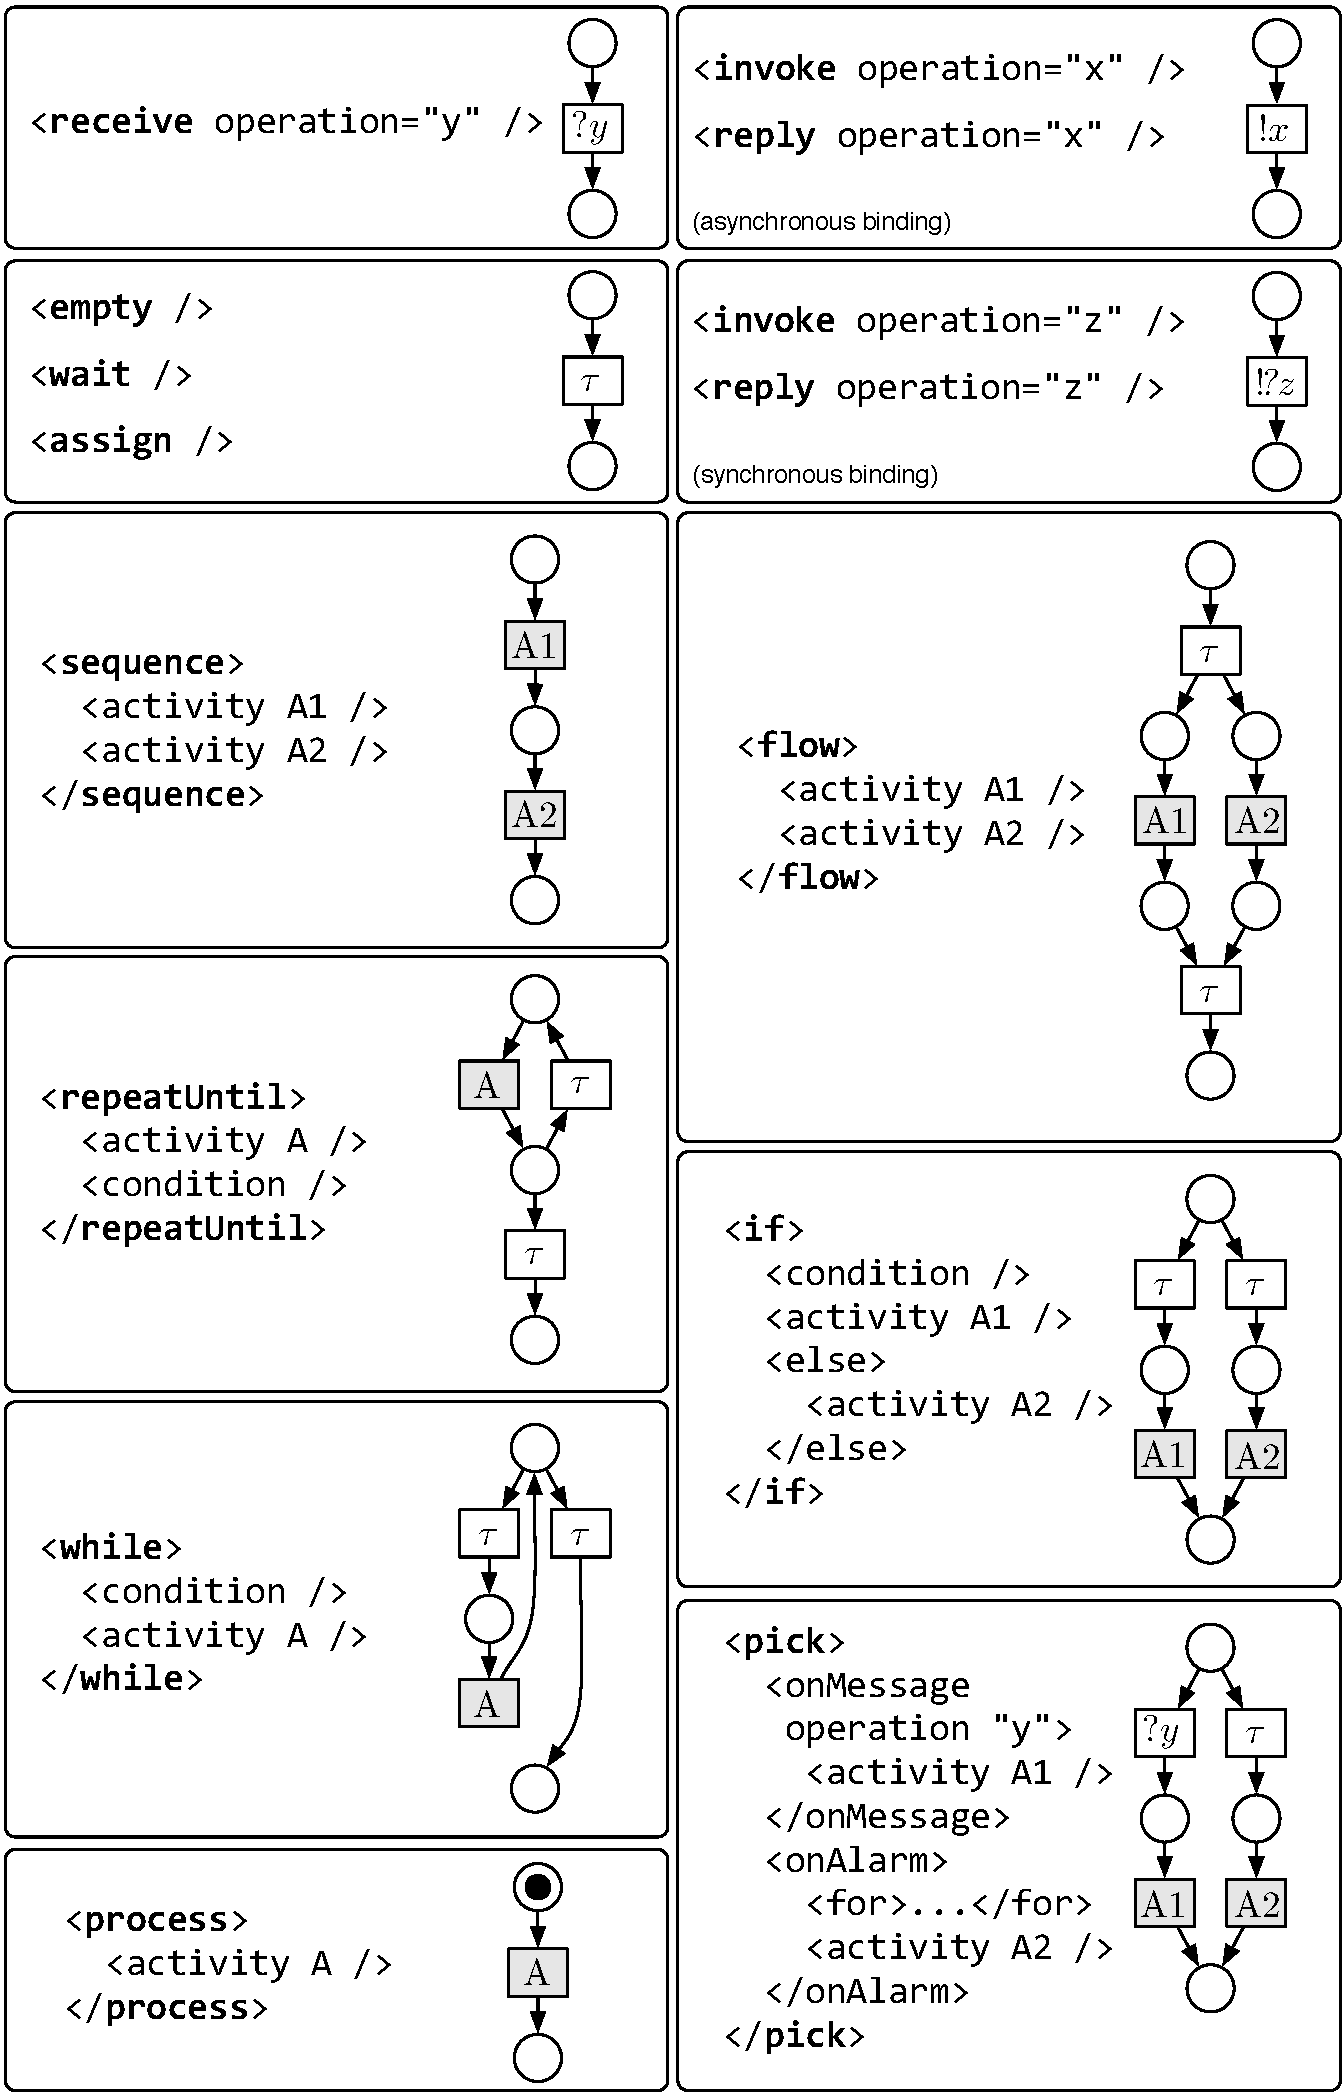
\includegraphics[scale=0.45]{verification/bpel}
\caption{Petri net patterns to formalize \acronym{WS-BPEL}.}\label{fig:bpel}
\end{figure}
%%%%%%%%%%%%%%%%%%%%%%%%%%%%%%%%%%%%%%%%%%%%%%%%%%%%%%%%%%%%%%%%%%%%%%%%%%%%%%

Whereas the original semantics~\cite{Lohmann_2007_wsfm,Lohmann_2007_hubtr212} captures the standard as well as the exceptional behavior of a \acronym{WS-BPEL} process, we only consider the standard behavior in this thesis to ease the presentation. We also do not present the formalization of control links and dead-path elimination. \Autoref{fig:bpel} gives an overview of the used patterns. These patterns can, however, be canonically enhanced to model fault, compensation, and exception handling of the participating \acronym{WS-BPEL} processes. The translation is guided by the structure of \acronym{WS-BPEL} and first translates the basic activities into the respective Petri net patterns. These nets are then embedded into those patterns structured activities. The interested reader is referred to a report~\cite{Lohmann_2007_hubtr212} which discusses the complete semantics as it is implemented in the tool \bpelowfn.

%%%%%%%%%%%%%%%%%%%%%%%%%%%%%%%%%%%%%%%%%%%%%%%%%%%%%%%%%%%%%%%%%%%%%%%%%%%%%%
\begin{figure}[tb]
\centering
\subfigure[service net with $\Omega=\{\mset{p_{\omega}}\}$\label{fig:verification:travelerpn}]{\makebox[0.49\textwidth]{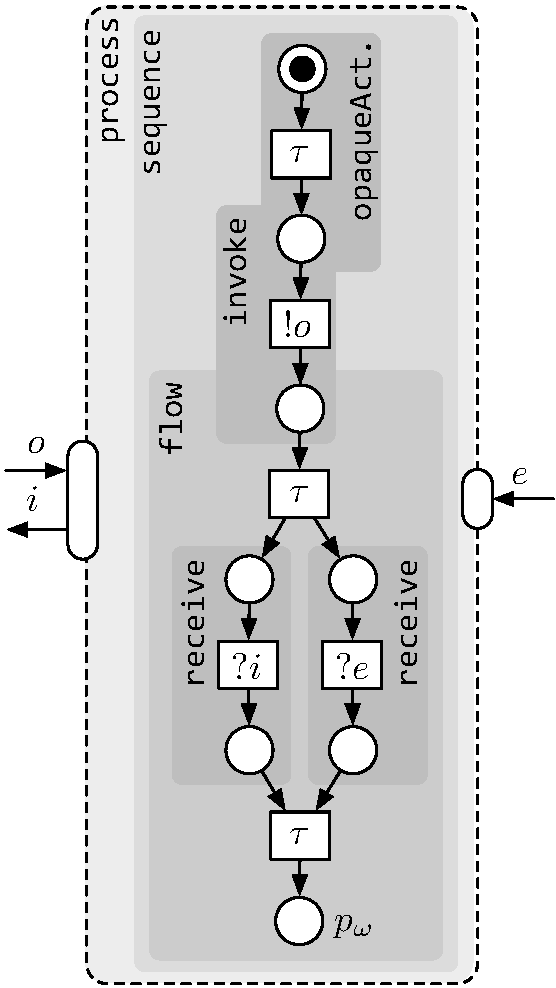
\includegraphics[scale=0.45]{verification/travelerpn}}}\hfill
\subfigure[corresponding service automaton\label{fig:verification:travelersa}]{\makebox[0.49\textwidth]{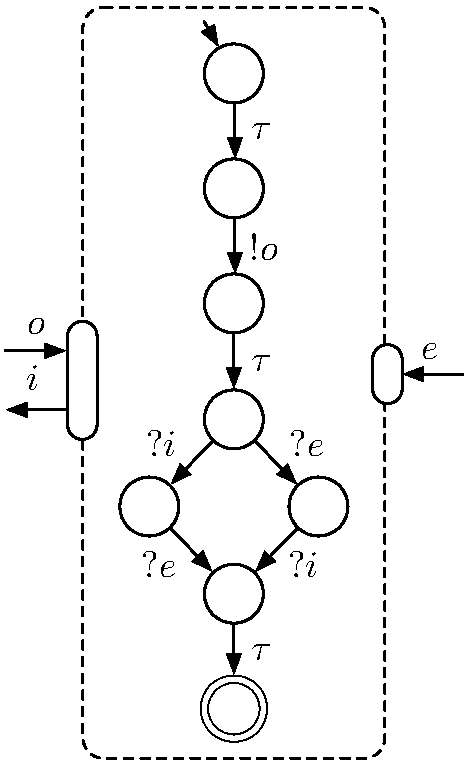
\includegraphics[scale=0.45]{verification/travelersa}}}
%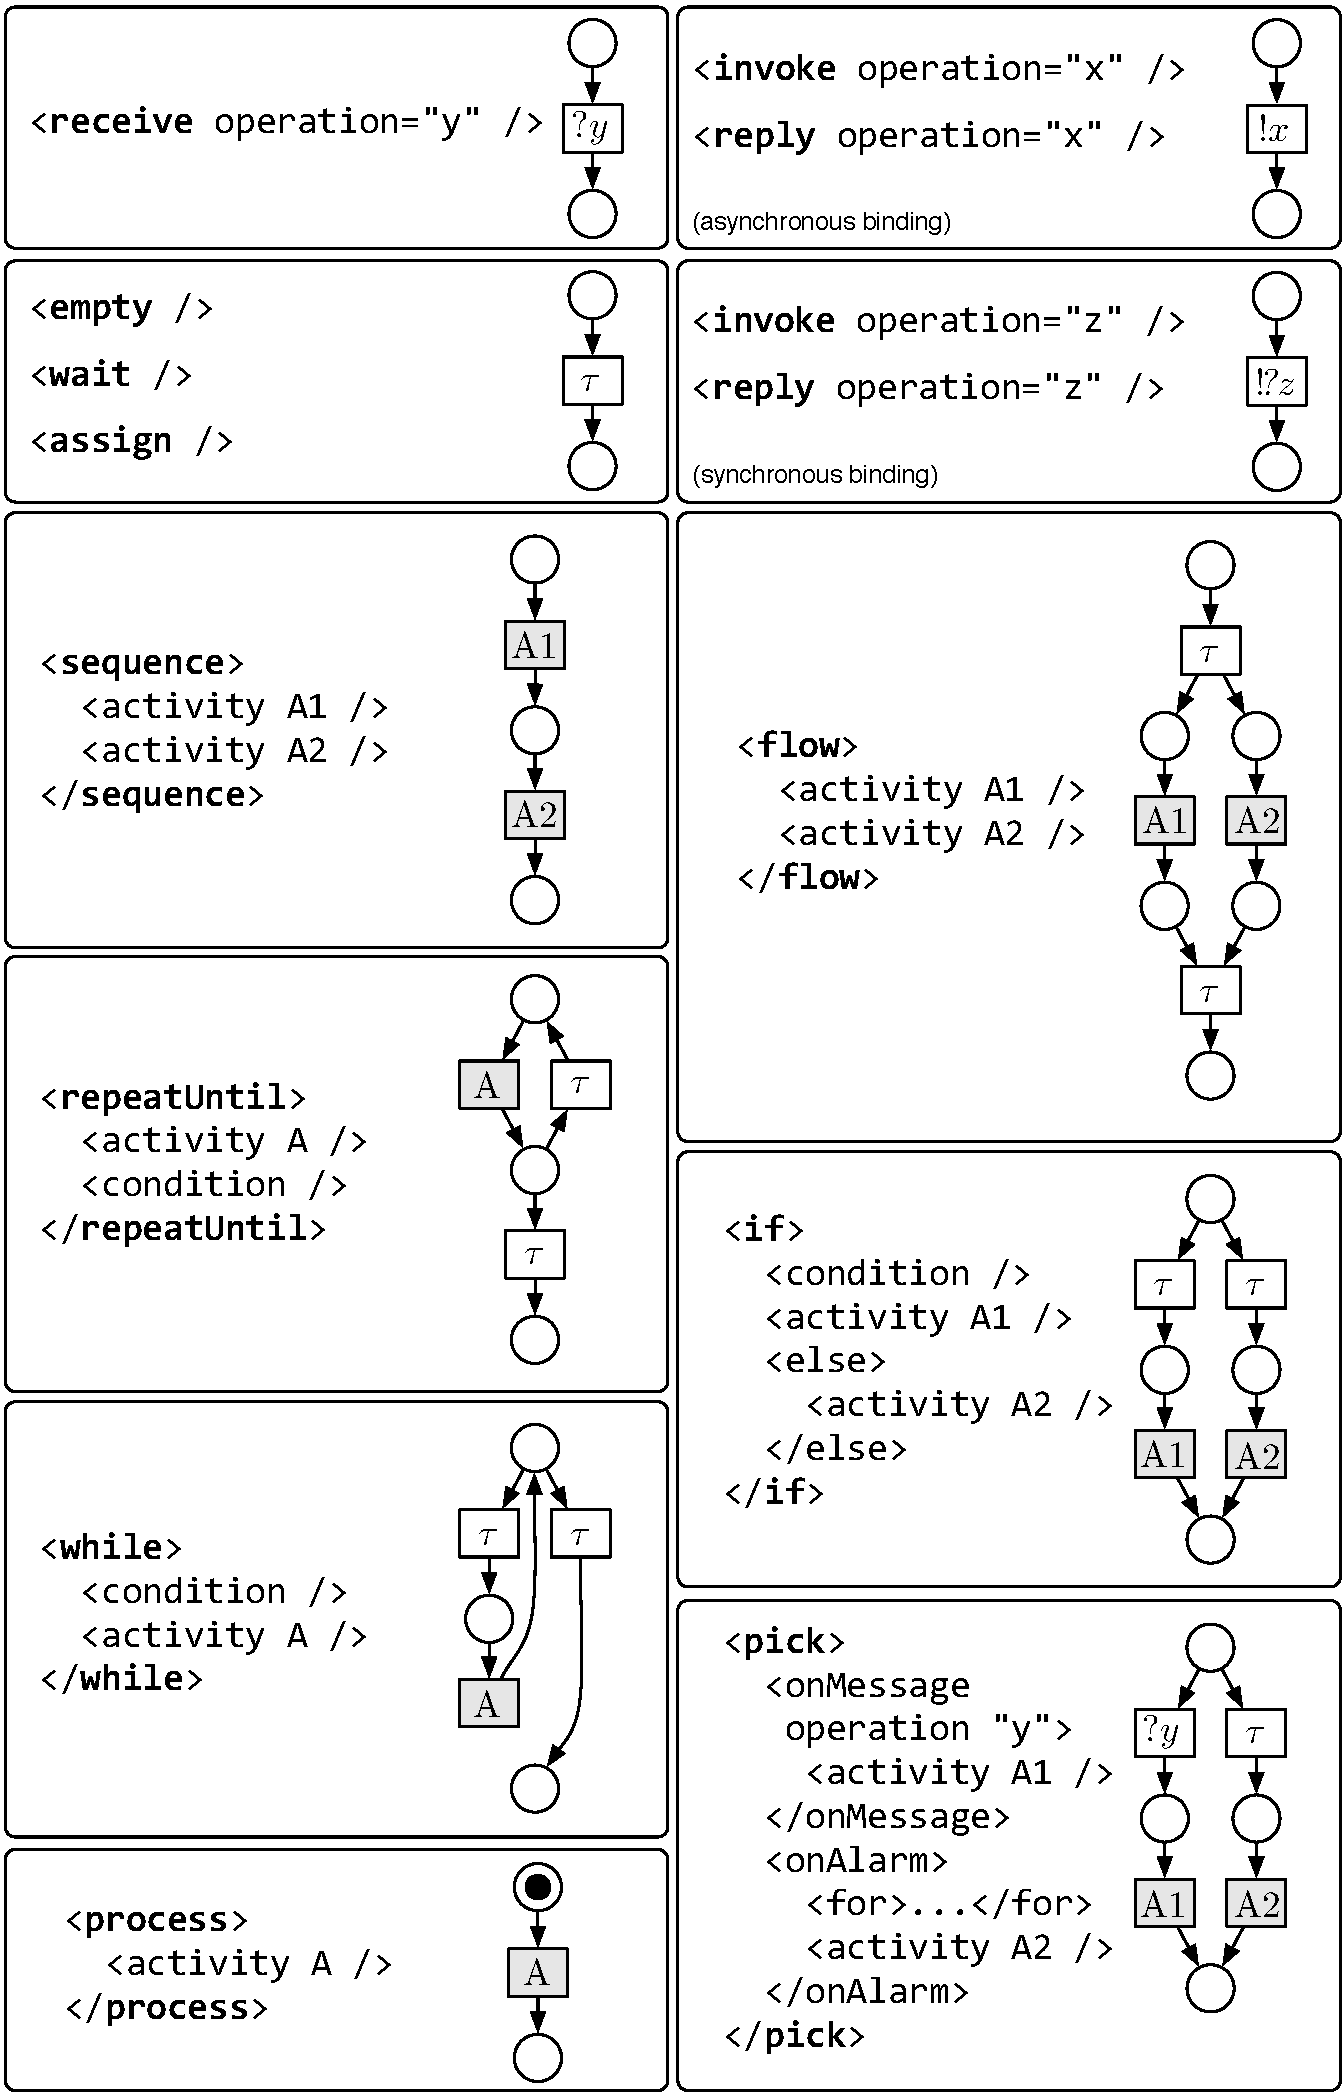
\includegraphics[scale=0.45]{verification/bpel}
\caption{Translation of the \acronym{WS-BPEL} traveler service.}\label{fig:verification:travelerpnsa}
\end{figure}
%%%%%%%%%%%%%%%%%%%%%%%%%%%%%%%%%%%%%%%%%%%%%%%%%%%%%%%%%%%%%%%%%%%%%%%%%%%%%%


\paragraph{Example.}

\Autoref{fig:verification:travelerpn} depicts the traveler service from \autoref{fig:verification:traveler} translated into a service net. From this net, a service automaton (cf.\ \autoref{fig:verification:travelersa}) can be canonically derived.




%%%%%%%%%%%%%%%%%%%%%%%%%%%%%%%%%%%%%%%%%%%%%%%%%%%%%%%%%%%%%%%%%%%%%%%%%%%%%%
\subsection*{Petri Net Semantics for BPEL{\footnotesize 4}Chor}

To translate a \bpelchor{} choreography, two steps are involved: (1) translate each participant's \acronym{WS-BPEL} process into a service automaton and (2) compose the resulting models. All required information can be derived from the \bpelchor{} choreography, cf.~\autoref{fig:artifacts}. In the ticket booking scenario we use as running example, however, there are several \emph{instances} of the airline service involved. To this end, the translation described in \cite{Lohmann_2007_wsfm,Lohmann_2007_hubtr212} needs to be extended to support multiple \emph{instantiation} of participants.

With ``instantiation'' we do not refer to the lifecycle of a service instance. This lifecycle includes the analysis of incoming messages to decide whether a new instance needs to be created or messages need to be forwarded to existing instances (called \emph{correlation} in \acronym{WS-BPEL}) and the removal of terminated instances from the execution engine. These steps are realized transparently by execution languages such as \acronym{WS-BPEL} and should not influence the behavior of a service composition. In the translation, ``instantiation'' means  creating several copies of a participants and adjusting the wiring of interfaces.

We realized the instantiation of a choreography participant by providing several identical copies of the service net of the participant description. By choosing unique place and transition names (\eg, using prefixes) the behavior of each instance is distinctively modeled. To be able to later compose these models, also the message channel names need to be adjusted to ensure bilateral and unidirectional communication. Therefore, we need to adjust the participant's behavior according to the following scenarios:

\begin{niceenumerate}
\item A message is exchanged between two uninstantiated participants (\eg, the trip order sent by the traveler to the agency): no adjustment is needed.

\item A message is exchanged between an uninstantiated participant and one particular instantiated participant (\eg, the price request sent by the agency to each airline instance): The behavior of the uninstantiated participant needs to be duplicated and executed for each instance, either concurrently or sequentially depending on the \bpel{forEach} activity used to traverse the instances. In addition, the message channel names need to be adjusted.

\item A message is exchanged between an uninstantiated participant and an arbitrary chosen instantiated participant (\eg, the e-ticket sent by the selected airline to the traveler): The behavior of the uninstantiated participant needs to be duplicated for each instance and executed mutually exclusively. In addition, the message channel names need to be adjusted.

\item A message is exchanged between two instantiated participants (not pre\-sent in our example choreography): Similar to the second scenario.
\end{niceenumerate}

As stated earlier, the participant topology holds the necessary information about which process and which message channel has to be instantiated. Admittedly, the topology does not provide the number of instances of each participant. \emph{We therefore demand an upper bound of instances to be specified for each participant set.} Whereas this upper bound may not be necessary if \bpelchor{} is just a means to \emph{describe} choreographies, its definition is reasonable if such a choreography should be \emph{analyzed} or \emph{executed}.

%%%%%%%%%%%%%%%%%%%%%%%%%%%%%%%%%%%%%%%%%%%%%%%%%%%%%%%%%%%%%%%%%%%%%%%%%%%%%%
\begin{figure}%[t!]
\centering
\subfigure[\label{fig:code} code snippet of the agency process]{\makebox[6cm]{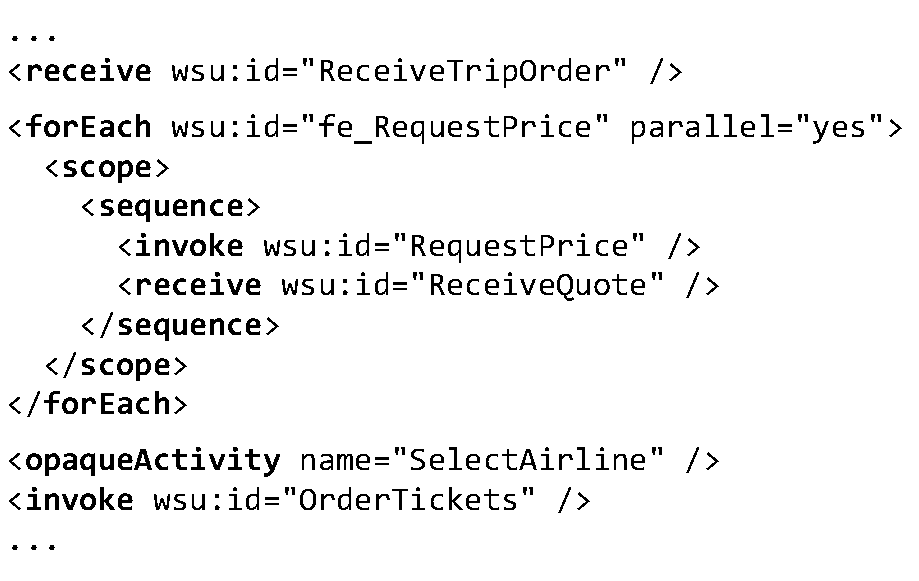
\includegraphics[scale=0.45]{verification/code}}}
\hfill
\subfigure[\label{fig:agency} resulting subnet of the agency]{\makebox[0.49\textwidth]{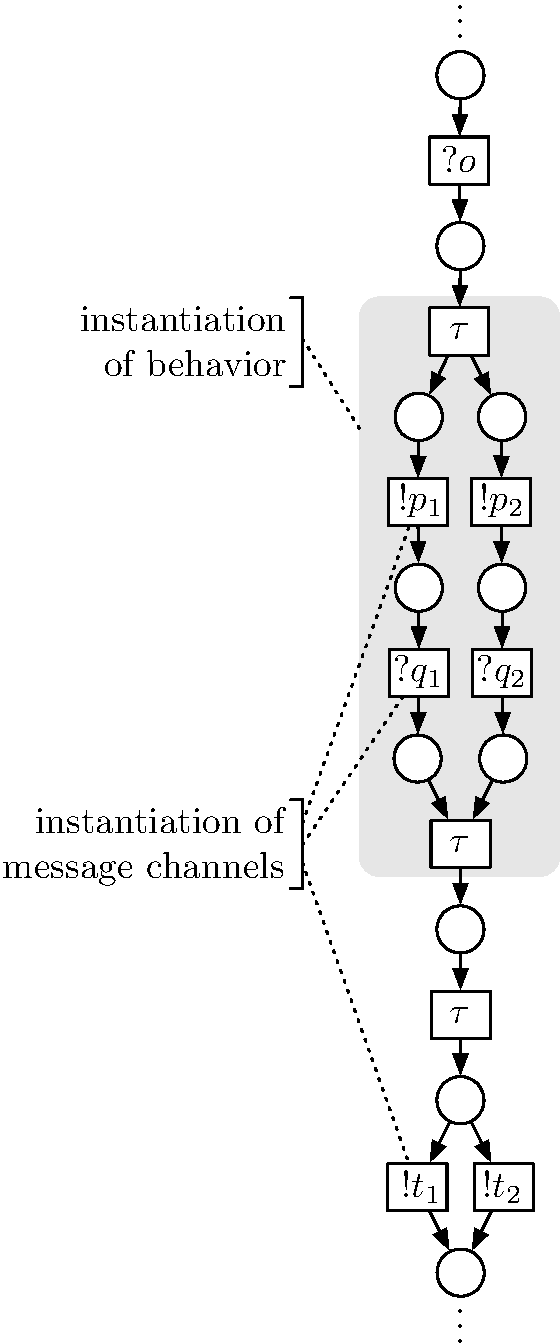
\includegraphics[scale=0.45]{verification/snippet_net}}}\subfigure[\label{fig:agencysa} resulting part as service automaton]{\makebox[0.49\textwidth]{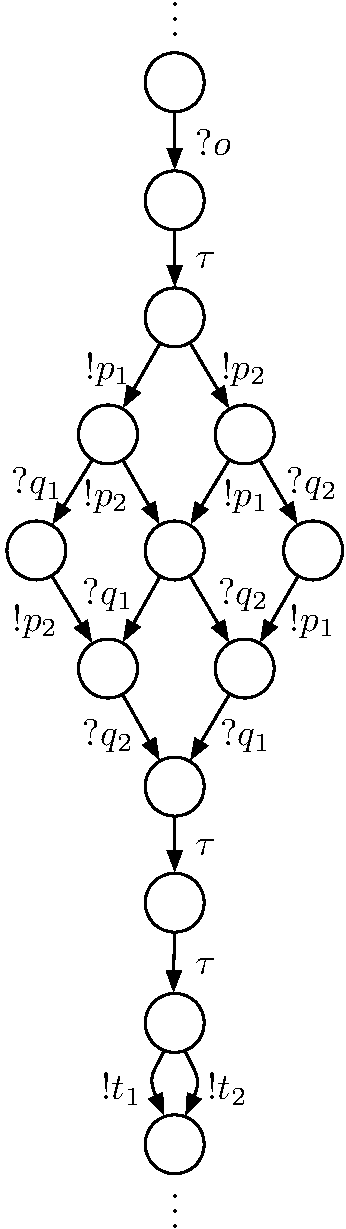
\includegraphics[scale=0.45]{verification/snippet_sa}}}
\caption{Example for the instantiation for two airline instances. The \acronym{WS-BPEL} process of the agency (a) translated into a Petri net (b) and a service automaton (c). }
\label{fig:instantiation}
\end{figure}
%%%%%%%%%%%%%%%%%%%%%%%%%%%%%%%%%%%%%%%%%%%%%%%%%%%%%%%%%%%%%%%%%%%%%%%%%%%%%%


\paragraph{Example.}

For an example of these scenarios, consider the \acronym{WS-BPEL} code snippet of the agency process depicted in \autoref{fig:code}. For two airline instances, \Autoref{fig:agency} depicts the resulting subnet. The trip order message ($o$) sent by the traveler to the agency is an example of the first scenario, as both services (traveler and agency) are uninstantiated. Therefore, the receipt of the trip order message is modeled by a single transition. The price request ($p_{1}$ and $p_{2}$) sent to and the corresponding price quotes ($q_{1}$ and $q_{2}$) received from the airline instances are examples for the second scenario. Therefore, the communicating transitions are instantiated, resulting in renamed message channel names. As specified by the parallel \bpel{forEach} activity, the agency communicates concurrently with each airline. The ticket order sent to only one airline instance ($t_{1}$ and $t_{2}$) is an example for the third scenario.




%%%%%%%%%%%%%%%%%%%%%%%%%%%%%%%%%%%%%%%%%%%%%%%%%%%%%%%%%%%%%%%%%%%%%%%%%%%%%%
\subsection*{Translating the example choreography}

The presented translation approach is implemented in our compiler \bpelowfn{} \cite{Lohmann_2007_hubtr212}. \bpelowfn\ enables us to automatically translate \acronym{WS-BPEL} choreographies into service net models. We translated the example choreography with 10 airline instances into a Petri net, cf.~\autoref{fig:choreography10}. The resulting net has 188 places and 151 transitions. Standard structural reduction techniques~\cite{Murata_1989_pieee} simplified the net to 113 places and 76 transitions while preserving compatibility.

%%%%%%%%%%%%%%%%%%%%%%%%%%%%%%%%%%%%%%%%%%%%%%%%%%%%%%%%%%%%%%%%%%%%%%%%%%%%%%
\begin{figure}[tb]
\centering
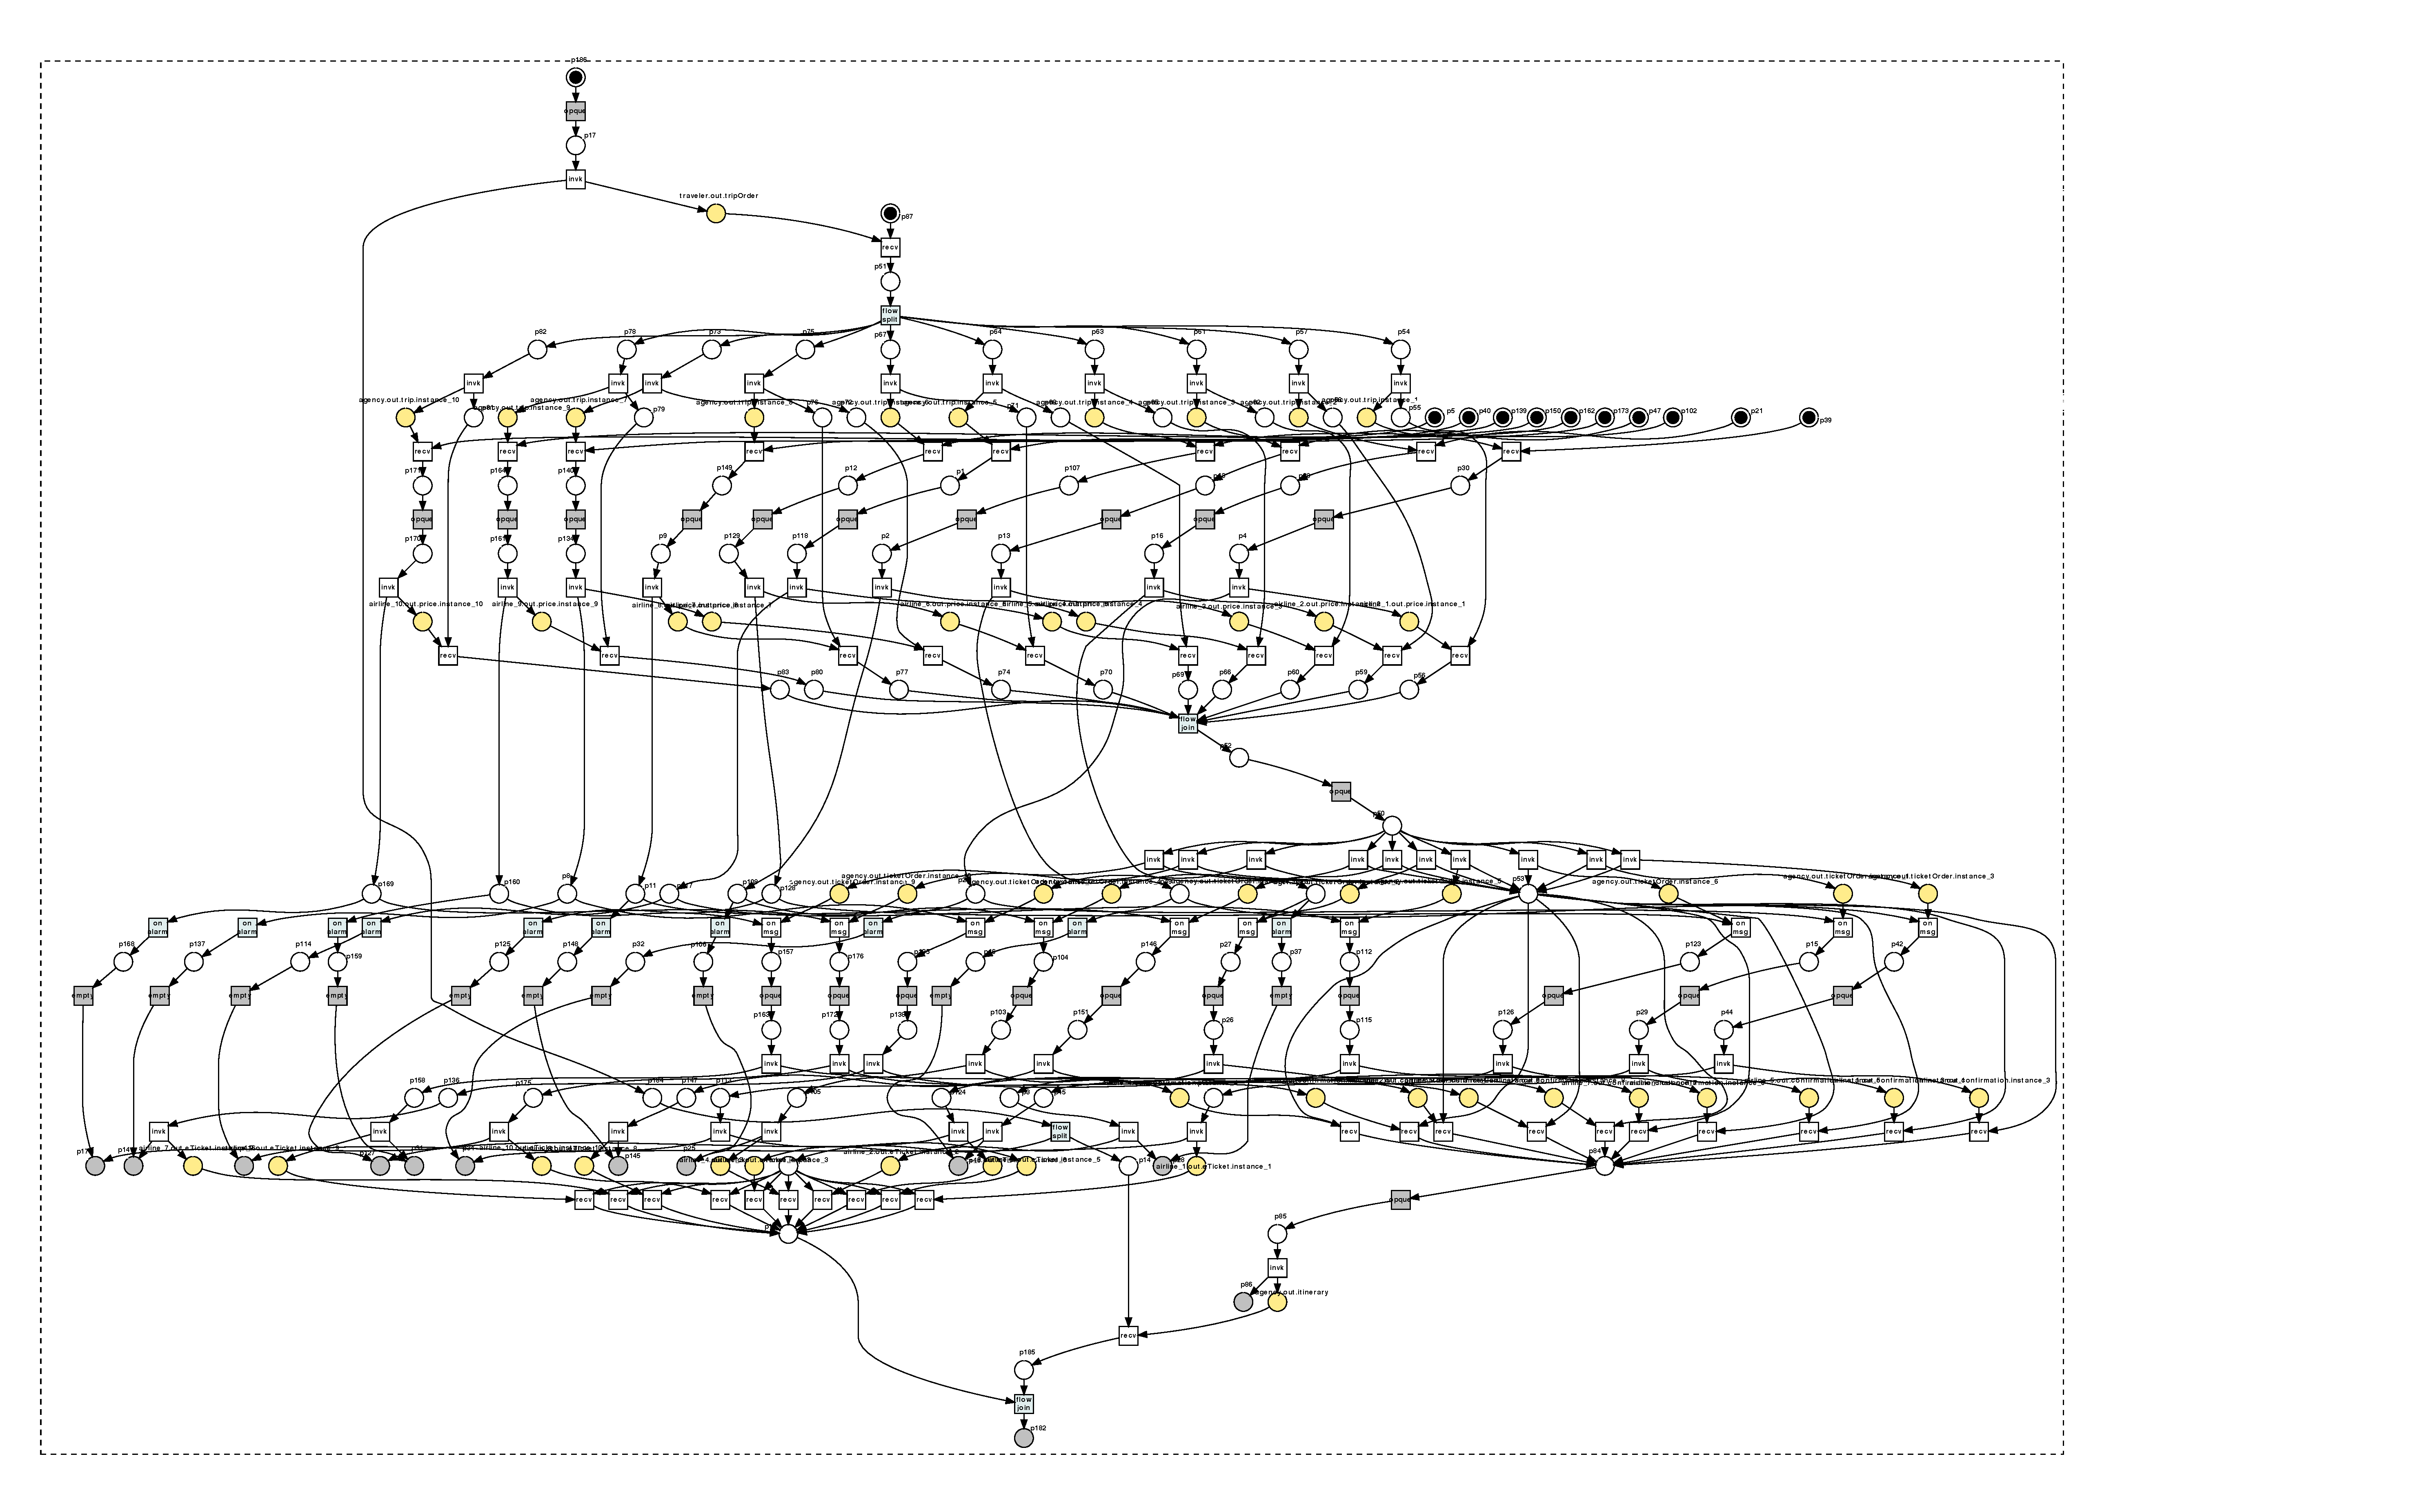
\includegraphics[width=0.9\textwidth]{verification/choreography10}
\caption{Service composition with 10 airline instances translated into a service net using the compiler \bpelowfn.}\label{fig:choreography10}%
\end{figure}
%%%%%%%%%%%%%%%%%%%%%%%%%%%%%%%%%%%%%%%%%%%%%%%%%%%%%%%%%%%%%%%%%%%%%%%%%%%%%%

In practice, we do not translate the intermediate \acronym{WS-BPEL} services into service automata, but compose the intermediate service nets. The definition of this service net composition operator is a straightforward adaption of \autoref{def:composition}; \citet{Wolf_2007_sa} provides a formal definition.





%%%%%%%%%%%%%%%%%%%%%%%%%%%%%%%%%%%%%%%%%%%%%%%%%%%%%%%%%%%%%%%%%%%%%%%%%%%%%%%
\section{Analyzing closed choreographies}\label{sec:Analysis}
%%%%%%%%%%%%%%%%%%%%%%%%%%%%%%%%%%%%%%%%%%%%%%%%%%%%%%%%%%%%%%%%%%%%%%%%%%%%%%%

A \bpelchor{} choreography description specifies not only the behavior of each participant, but also their interaction. In addition, the \mbox{closed-world} assumption ensures that there is no further entity influencing the behavior of the participants. As a result, a complete \bpelchor{} choreography description can be translated into a closed service automaton (\ie, a service automaton with closed interface). Such a closed system can be analyzed without the necessity of taking an environment into account.

The correctness of a \bpelchor{} choreography is crucial, because it is the basis for technical groundings as well as manual refinement (cf.~\autoref{fig:bpelchortrans}). By checking this \bpelchor{} choreography, we can rule out errors well before refinement, implementation, and deployment.

As motivated in \autoref{chap:formal}, we employ compatibility as central correctness criterion for closed service compositions. It allows us to derive more elaborate concepts such as controllability, behavioral constraints, or operating guidelines. Beside compatibility, temporal logics allow to express several other properties of closed systems which can be investigated using standard model checking tools~\cite{ClarkeGD_1999_book,BaierK_2008_book}. Interesting questions include:

\begin{niceitemize}
\item Will a certain activity of a participant be executed?

\item Does there exist a state in which more than one message is pending on a communication channel? 

\item What is the minimal/maximal number of messages to be sent to reach a final state of the choreography?

\item Will a participant always receive an answer? Can a participant enforce the receipt of a certain message?
\end{niceitemize}

These properties focus on closed systems and are not applicable to open systems in which an environment has to be taken into account. In this situation, the application of behavioral constraints (cf.~\autoref{chap:validation}) may help to investigate and validate the participants' behavior, but the results cannot be straightforwardly mapped back to the original \acronym{WS-BPEL} or \bpelchor{} model.




%%%%%%%%%%%%%%%%%%%%%%%%%%%%%%%%%%%%%%%%%%%%%%%%%%%%%%%%%%%%%%%%%%%%%%%%%%%%%%
\subsection*{Analyzing the example choreography}

We analyzed the Petri net model of Sect.~\ref{sec:Translation} with the Petri net verification tool LoLA~\cite{Schmidt_2000_icatpn,Wolf_2007_icatpn}, a state-of-the-art model checker which implements several state space reduction techniques. The unreduced state space consists of 9{,}806{,}583 states. Using LoLA, we detected a deadlock in the model. We could map this deadlocking state of the model back to the participating services with the help of a \emph{witness path}. The deadlock occurs, if the agency's choice for an airline takes too much time or if the message sent to the chosen airline is delayed. In this case, the timeout (\ie, the \bpel{onAlarm} branch) of \emph{all} participating airlines ends their instances and the agency deadlocks waiting for a confirmation message from the chosen airline.

Even though the presented example does not have the complexity of industrial service choreographies, the design flaw is very subtle and was not detected by the authors of the paper~\cite{DeckerKLW_2007_icws}, where the example was taken from. Admittedly, our formalization abstracted from time and models timer-based decisions by nondeterminism. Nevertheless, the detected deadlock models a situation in which all airline instances time out, which may happen independently of a concretely chosen timeout interval. In addition, the latency of messages is hard to predict when asynchronous message transfer over the Internet is used to interact.




%%%%%%%%%%%%%%%%%%%%%%%%%%%%%%%%%%%%%%%%%%%%%%%%%%%%%%%%%%%%%%%%%%%%%%%%%%%%%%
\subsection*{Correcting the example choreography}

There are many ways to correct the deadlocking choreography. A straightforward attempt would be to replace the airline service's timeout by a message sent by the agency, which explicitly informs all but one airline that their price quote was not chosen. This would, however, add an unrealistic dependency between the agency and all running airline instances. To this end, we decided to keep the timeout, but at the same time ensure a response of the airline service even if a ticket order is received after the timeout.

%%%%%%%%%%%%%%%%%%%%%%%%%%%%%%%%%%%%%%%%%%%%%%%%%%%%%%%%%%%%%%%%%%%%%%%%%%%%%%
\begin{figure}
\centering
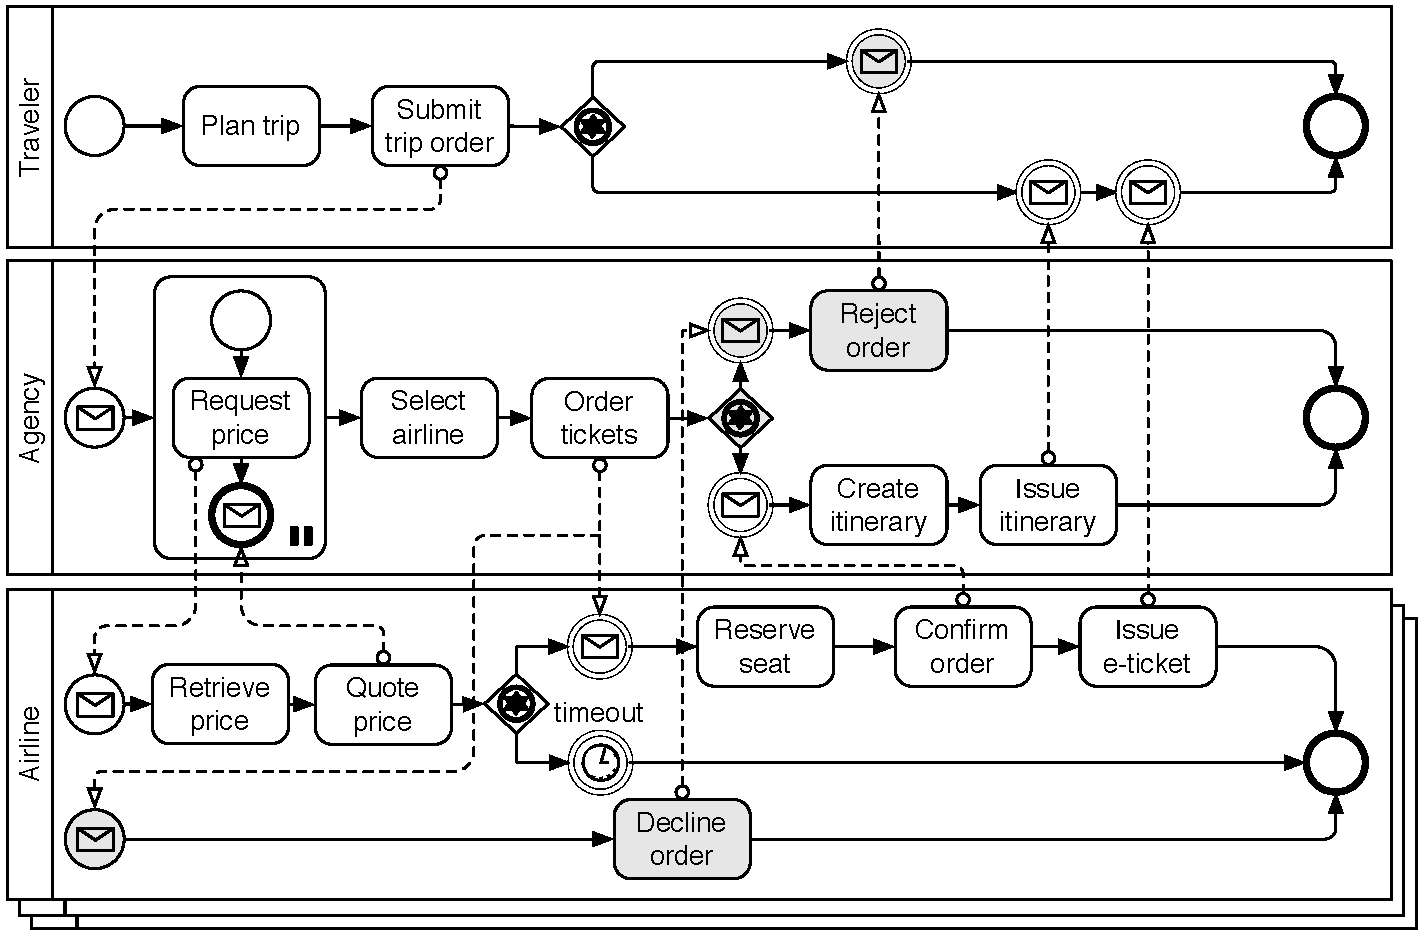
\includegraphics[scale=0.45]{verification/choreo-fix}
\caption{Fixed choreography of the ticket booking scenario. The two start events at the airline process denote a \acronym{WS-BPEL} \bpel{pick} activity.} \label{fig:fixed}
\end{figure}
%%%%%%%%%%%%%%%%%%%%%%%%%%%%%%%%%%%%%%%%%%%%%%%%%%%%%%%%%%%%%%%%%%%%%%%%%%%%%%

Hence, we changed the choreography as follows (cf.~gray shapes in \autoref{fig:fixed}). The airline's behavior does not change if the agency's ticket order is received before the timeout occurred and if the timeout occurs, the airline service's instance still terminates. However, a new branch was added to the airline: \emph{this branch models the situation in which the agency's ticket order is received after the timeout. In this case, the airline service is restarted and the ticket order is rejected.} In addition, the services of the agency and the traveler are adjusted to handle the case in which all airlines time out and no ticket could be booked.

Note that \acronym{BPMN} can only specify message flow between exactly two activities and does not support the concept of message channels. In the fixed choreography however, the ticket order sent by the agency can be received by two message events of the airline. We denote this in \autoref{fig:fixed} by a branching message flow originating in the ``order tickets'' activity of the travel agency.




%%%%%%%%%%%%%%%%%%%%%%%%%%%%%%%%%%%%%%%%%%%%%%%%%%%%%%%%%%%%%%%%%%%%%%%%%%%%%%
\subsection*{Analyzing the fixed example choreography}

We translated the fixed choreography with five airline instances into a Petri net model. Because of the newly introduced activities, its structure and its state space have grown. The resulting (structurally reduced) net has 113 places and 97 transitions. The model has 9{,}805{,}560 states and is now compatible.

\medskip

The correction is nontrivial and possibly error-prone. To ensure compatibility, an additional check is needed. In the next chapter, we shall provide an algorithm to automatically suggest corrections for incorrect choreographies.



%%%%%%%%%%%%%%%%%%%%%%%%%%%%%%%%%%%%%%%%%%%%%%%%%%%%%%%%%%%%%%%%%%%%%%%%%%%%%%%
\subsection*{Experimental results}

In the previous sections, we analyzed the first and the second choreography (cf.~\autoref{fig:broken} and \autoref{fig:fixed}, resp.) with five airline instances. For these five airlines, the resulting models already had more than 3{,}000 states. The states space grows dramatically when the number of airlines is further increased (cf.~\autoref{tab:verification_sizes}). For ten airlines, the model has over nine million states, and for larger numbers, the full state space could not be constructed due to memory overflow (denoted by ``---'' in \autoref{tab:verification_sizes}). The experiments conducted using a computer with 2 gigabytes of memory.

%%%%%%%%%%%%%%%%%%%%%%%%%%%%%%%%%%%%%%%%%%%%%%%%%%%%%%%%%%%%%%%%%%%%%%%%%%%%%%
\begin{table}
\centering
\caption{Experimental results for compatibility check using LoLA.}
\medskip
\label{tab:verification_sizes}
first example, cf.~\autoref{fig:broken} \footnotesize
\begin{tabular*}{\textwidth}{@{\extracolsep{\fill}}lrrrrr}
\toprule
airline instances & $1$ & $5$ & $10$ & $100$ & $1{,}000$\\ \midrule
net places & $20$ & $63$ & $113$ & $1{,}013$ & $10{,}013$ \\
net transitions & $10$ & $41$ & $76$ & $706$ & $7.006$ \\ \midrule
states (unreduced) & $14$ & $3{,}483$ & $9{,}806{,}583$ & --- & ---  \\
states (symmetry) & $14$ & $561$ & $378{,}096$ & --- & ---  \\
states (POR) & $11$ & $86$ & $261$ & $18{,}061$ & $1{,}752{,}867$  \\
states (POR + symmetry) & $11$ & $30$ & $50$ & $410$ & $4{,}010$  \\
\bottomrule
\end{tabular*}
\medskip\\
\normalsize second example, cf.~\autoref{fig:fixed}\\ \footnotesize
\begin{tabular*}{\textwidth}{@{\extracolsep{\fill}}lrrrrr}
\toprule
airline instances & $1$ & $5$ & $10$ & $100$ & $1{,}000$ \\ \midrule
net places & $19$ & $63$ & $113$ & $1{,}013$ & $10{,}113$ \\
net transitions & $12$ & $52$ & $97$ & $907$ & $9{,}007$ \\ \midrule
states (unreduced) & $13$ & $3{,}812$ & $9{,}805{,}560$ & --- & --- \\
states (symmetry) & $13$ & $704$ & $329{,}996$ & --- & --- \\
states (POR) & $12$ & $88$ & $228$ & $8{,}361$ & $734{,}049$ \\
states (POR + symmetry) & $12$ & $28$ & $43$ & $314$ & $3{,}014$ \\
\bottomrule
\end{tabular*}
\end{table}
%%%%%%%%%%%%%%%%%%%%%%%%%%%%%%%%%%%%%%%%%%%%%%%%%%%%%%%%%%%%%%%%%%%%%%%%%%%%%%

However, several state space reduction techniques can be applied to reduce the size of the state space while still being able to analyze desired properties such as deadlock-freedom. In our particular example, we applied \emph{symmetry reduction} and \emph{partial order reduction}, both implemented in LoLA (\citet{Wolf_2007_icatpn} provides further references). The symmetry reduction exploits  that all airline instances have the same structure. This regular structure induces symmetries on the net structure itself, but also on the state space of the choreography. Intuitively, the instances of the airline service act ``similar'' or ``symmetric''. During the state space construction, symmetric states are merged. The partial order reduction follows a different approach: As all instances run concurrently, any order of transitions of the airline instances are represented in the state space. These transition sequences introduce an exponential number of intermediate states, resulting in state space explosion. However, the actual order of independent actions is not relevant to detect deadlocks, for instance. To this end, partial order reduction tries to only construct a single transition sequence of transitions of different airline instances to ease the state space explosion.

\enlargethispage*{\baselineskip}

In case each of the reduction technique is applied in isolation, the number of states grows more slowly, yet still exponentially in the number of airline instances. The combination of both techniques, however, yields a linear increase of states (cf.~\autoref{tab:verification_sizes}). Hence, we are able to verify properties of \acronym{WS-BPEL} choreographies with thousands of participating services. This shows that the presented approach should be likewise suitable to analyze real-life examples. The numbers show that the correction of the model only yields few additional states.





%%%%%%%%%%%%%%%%%%%%%%%%%%%%%%%%%%%%%%%%%%%%%%%%%%%%%%%%%%%%%%%%%%%%%%%%%%%%%%%
\section{Completing Choreographies}\label{sec:ver:syn}
%%%%%%%%%%%%%%%%%%%%%%%%%%%%%%%%%%%%%%%%%%%%%%%%%%%%%%%%%%%%%%%%%%%%%%%%%%%%%%%

While the analysis of closed choreographies may help to find errors such as deadlocks in the interaction between the participating services, service automata may also support the \emph{design} of choreographies. A choreography in which one participating service is missing can, for instance, be \emph{completed} by automatically synthesizing the missing participant service. This synthesized service is then guaranteed to communicate compatibly with the other participants. To this end, controllability is an important property. In~\autoref{chap:formal}, we presented an algorithm to constructively decide controllability of an open service automaton. This algorithm is implemented in the tool Wendy~\cite{LohmannW_2009_wendy}. If a partner exists such that the composition is compatible, it is automatically generated.




%%%%%%%%%%%%%%%%%%%%%%%%%%%%%%%%%%%%%%%%%%%%%%%%%%%%%%%%%%%%%%%%%%%%%%%%%%%%%%
\subsection*{Synthesizing a traveler participant}

Consider again the fixed choreography of \autoref{fig:fixed}. If, for example, only the services of the agency and the airlines were specified, the blueprint of a traveler participant could be synthesized. If such a service exists (\ie, the composition of the existing services is controllable), it completes the choreography which is then compatible by construction. To this end, the incomplete choreography is translated into a service net using \bpelowfn. This service automaton is then analyzed by Wendy. If the service automaton is controllable, a service automaton modeling the behavior of a partner service is synthesized.

%%%%%%%%%%%%%%%%%%%%%%%%%%%%%%%%%%%%%%%%%%%%%%%%%%%%%%%%%%%%%%%%%%%%%%%%%%%%%%
\begin{figure}[tb]
\centering
\subfigure[synthesized traveler\label{fig:synthesized_traveler}]{\makebox[0.45\textwidth]{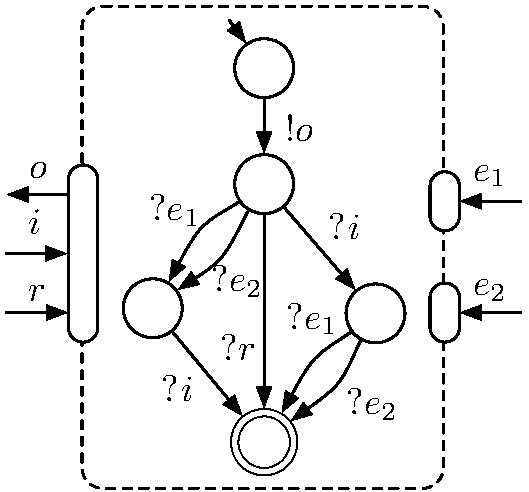
\includegraphics[scale=0.45]{verification/syn_traveler}}}\hfill
\subfigure[two synthesized airline instances\label{fig:synthesized_airlines}]{\makebox[0.45\textwidth]{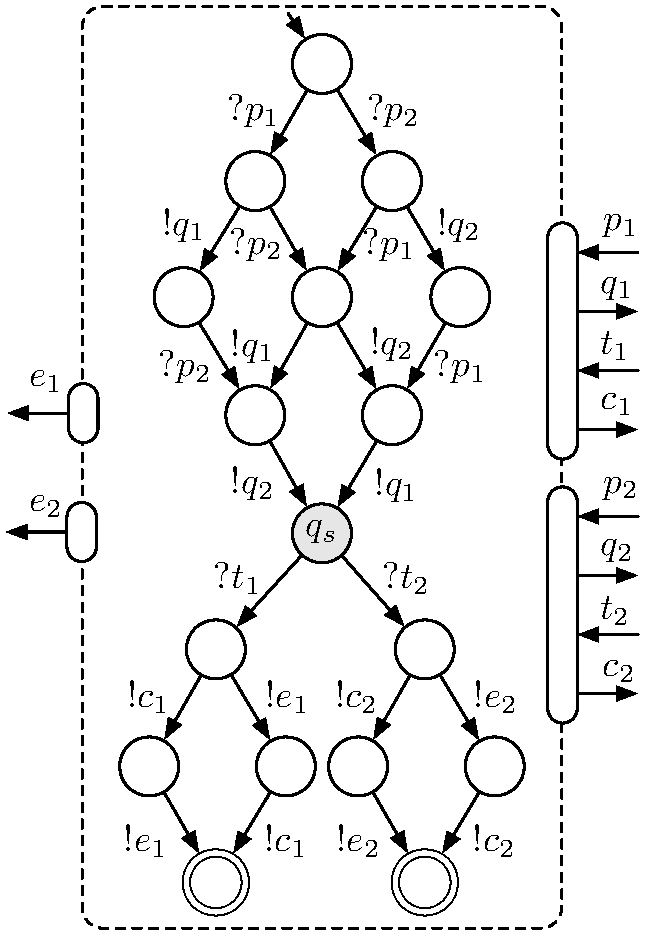
\includegraphics[scale=0.45]{verification/syn_airline}}}
\caption{Participant services synthesized to complete the example choreography.}
\end{figure}
%%%%%%%%%%%%%%%%%%%%%%%%%%%%%%%%%%%%%%%%%%%%%%%%%%%%%%%%%%%%%%%%%%%%%%%%%%%%%%


\paragraph{Example.}

\Autoref{fig:synthesized_traveler} depicts the synthesized service automaton of a traveler participant which completes the choreography. This traveler participant slightly differs from the traveler participant in the repaired choreography (cf.~\autoref{fig:fixed}). First, there exists no transition modeling the planning of the trip, because such a transition is internal (\ie, not communicating), but the participant was synthesized based on the external behavior; that is, only the interaction of the service was taken into account. Second, the itinerary and the e-ticket can be received in any order. For example, it would be possible to swap the two receive events in~\autoref{fig:fixed}. This is because of the asynchronous communication model: messages can keep pending on the interface, so there is no order in which they have to be received. From this service automaton, an abstract \acronym{WS-BPEL} process can be derived using existing approaches~\cite{LassenA_2006_otm,AalstL_2008_ist,LohmannK_2008_mod}. As this translation is out of scope of this thesis, we do not present it here.




%%%%%%%%%%%%%%%%%%%%%%%%%%%%%%%%%%%%%%%%%%%%%%%%%%%%%%%%%%%%%%%%%%%%%%%%%%%%%%
\subsection*{Experimental results}

To investigate the applicability of the synthesis algorithm in this scenario, we conducted the following experiment. We fixed the travel agency and synthesized the traveler service for different numbers of airline instances.

\Autoref{tab:syn} summarizes the results. The first two lines list the size of the structurally reduced service net modeling the composition of the airline instances and the travel agency. The next line lists the number of states of this open composition; that is, the size of the service automaton that is checked for controllability. The next two lines give information on the size of the synthesized traveler service. Finally, the time consumption of the synthesis is listed. With our test setup of 2 gigabytes of memory and a 3 \acronym{GH}z processor, we were able to synthesize a traveler service for up to 14 airline instances. For this number, the service automaton modeling the composition of the travel agency and the airline instances has already more than five million states and the synthesis took more than six minutes.

%%%%%%%%%%%%%%%%%%%%%%%%%%%%%%%%%%%%%%%%%%%%%%%%%%%%%%%%%%%%%%%%%%%%%%%%%%%%%%
\begin{table}
\centering
\caption{Experimental results for participant synthesis using Wendy.}
\medskip
\label{tab:syn}
\footnotesize
\begin{tabular*}{\textwidth}{@{\extracolsep{\fill}}lrrrrrr}
\toprule
airline instances  & $4$ & $6$ & $8$ & $10$ & $12$ & $14$ \\ \midrule
net places       & $35$ & $49$ & $63$ & $77$ & $91$ & $105$ \\
net transitions  &$18$ & $26$ & $34$& $42$& $50$& $58$  \\
states  & $176$ & $1{,}240$ & $9{,}120$ & $71{,}366$ & $588{,}784$ & $5{,}045{,}112$ \\ \midrule
synthesized states  & $11$ & $15$ & $19$ & $23$ & $27$ & $31$\\
synthesized transitions  & $56$ & $106$ & $172$ & $254$ & $352$ & $466$ \\
synthesis time [s] & $0$& $0$ & $0$ & $3$ & $36$ & $378$ \\
\bottomrule
\end{tabular*}
\end{table}
%%%%%%%%%%%%%%%%%%%%%%%%%%%%%%%%%%%%%%%%%%%%%%%%%%%%%%%%%%%%%%%%%%%%%%%%%%%%%%

Compared with the compatibility analysis (cf.~\autoref{tab:verification_sizes}), the synthesis problem does not scale well with respect to the number of airline instances that can be processed (14 vs.\ 1{,}000). This is because we currently do not apply state space reduction techniques. Hence, the size of the service automaton to be considered suffers from state explosion and grows exponentially in the number of the airline instances. However, without these techniques, also the compatibility analysis becomes unfeasible if the size of the state space exceeds about 10 million states.

The experiment also shows that just a small number of asynchronously communicating participants are enough to result in an open system which has much more states than industrial Web services (cf.~\autoref{tab:synthesis}). For the ticket booking scenario, the composition of a travel agency and ten airline instances has already four times more states than the largest service automaton we considered in~\autoref{tab:synthesis}.




%%%%%%%%%%%%%%%%%%%%%%%%%%%%%%%%%%%%%%%%%%%%%%%%%%%%%%%%%%%%%%%%%%%%%%%%%%%%%%
\subsection*{Limits of the participant synthesis}

The approach presented allows us to synthesize a participant that interacts in a compatible manner with the other participating services of the choreography. This is, of course, only possible if the open choreography is controllable and thus such a service exists. Currently, it is, however, not possible to synthesize a \emph{set} of services which complete a choreography: \autoref{def:synthesis} synthesizes a single strategy. First ideas toward and extension of the synthesis algorithm to multiple services are described by \citet{Wolf_2008_topnoc}. We shall come back to this in \autoref{chap:realizability}.

As an example, consider again the first (deadlocking) choreography in \autoref{fig:broken}. The choreography deadlocks because of the airline service's timeout mechanism. If we synthesize a strategy for the composition of the traveler and the travel agency, the result will be a \emph{single} service automaton modeling the behavior of \emph{all} airline service's instances. \Autoref{fig:synthesized_airlines} depicts this service automaton modeling two airline instances. It receives two price requests from the agency addressed to the different instances ($p_{1}$ and $p_{2}$) which reply with two price quotes ($q_{1}$ and $q_{2}$). Then, it waits to receive a ticket order (either $o_{1}$ or $o_{2}$) and answers it accordingly (either $c_{1}$ or $c_{2}$). The resulting choreography would be compatible. However, the airline's instances are not independent of each other. They are implicitly synchronized in state $q_{s}$ (depicted gray in \autoref{fig:synthesized_airlines}): after this state, only one of the airlines continues the interaction. If this service had to be split into two services (one for each instance), this synchronization would have to be made  explicit by adding coordination messages to maintain compatibility. Still, the synthesized airline model can be seen as a starting point for further refinement. In the next chapter, we shall use synthesized strategies as a starting point to automatically propose correction for incompatible compositions. We shall again consider the resolution of dependencies between different choreography participants in \autoref{chap:realizability} when we study interaction models.

\medskip

\enlargethispage*{\baselineskip}

Another aspect of the participant synthesis is the \emph{causality} between messages. As sketched in the description of the generated traveler participant (cf.~\autoref{fig:synthesized_traveler}), a generated participant may send and receive messages in different\,--- \,typically less constrained\,---\,orders. This may yield synthesized services which send acknowledgment messages before actually receiving the corresponding request. In such cases, the causality between the request and the acknowledgment is ignored. Such causal effects have been studied by \citet{Wolf_2008_topnoc} who further considers semantics of messages~\cite{Wolf_2008_awpn}. In \autoref{chap:validation}, we introduced behavioral constraints to rule out such implausible behavior.





%%%%%%%%%%%%%%%%%%%%%%%%%%%%%%%%%%%%%%%%%%%%%%%%%%%%%%%%%%%%%%%%%%%%%%%%%%%%%%%
\section{Related Work}\label{sec:ver:related}
%%%%%%%%%%%%%%%%%%%%%%%%%%%%%%%%%%%%%%%%%%%%%%%%%%%%%%%%%%%%%%%%%%%%%%%%%%%%%%%

As described in the introduction, choreography models can be grouped into interconnected models and interaction models. In this chapter, we only considered the former. We shall consider interaction models in \autoref{chap:realizability}.


\paragraph{WS-BPEL and BPEL{\footnotesize 4}Chor.}

There exists a large number of formalizations of\break \acronym{WS-BPEL} (see \cite{BreugelK2006,LohmannVOSA_2009_ijbpim,LohmannVD_2008_topnoc} for surveys) which can all be similarly adjusted to model \bpelchor{} as long as they formalize the exchange of messages. \citet{DeckerKLW_2009_dke} give a detailed evaluation of existing choreography languages and an assessment of the features of \bpelchor{}. Whereas we use \acronym{BPMN} for visualization purposes only, \citet{DeckerKLPW_2008_caise} provide an extension to \acronym{BPMN} to specify complete \bpelchor{} choreography using \acronym{BPMN}.


\paragraph{Analysis.}

Compatibility of service compositions and service choreographies has already received much attention in the early days of Web services~\cite{YellinS_1997_toplas,NarayananM_2002_www,Rachid-Hamadi_2003_adc,BultanFHS_2003_www,Foster_UMK04_icws,Martens_2005_fase, PuhlmannW_2006_icsoc,DeckerW_2007_caise}. Compatibility of a closed composition is closely related to\,---\,and motivated by\,---\,the \emph{soundness} property of workflows~\cite{Aalst_1998_jcsc,VerbeekBA_2001_tcj}. For soundness, a case study~\cite{FahlandWJKLVW_2009_bpm} shows that industrial process models can already be checked in few milliseconds using the tool LoLA. Beside verification, \citet{Mendling_2008_phd} applied empirical studies to \emph{predict} errors in process models from the structure and the used language constructs.

\citet{MoserMHM06} show how to synthesize a \acronym{WS-BPEL} process which properly interacts with a given \acronym{WS-BPEL} process.
\citet{DeckerKP_2007_yrsoc} present a formalization of \bpelchor{}, focusing on \emph{service referrals} (also called link passing). They provide a mapping to the $\pi$-calculus, but give no details on possible verification.


\paragraph{Refinement.}

The refinement from a grounded \bpelchor{} choreography to executable \acronym{WS-BPEL} processes has two aspects. On the one hand, technical details such as \acronym{WSDL} port types or data types have to be added to the participant descriptions. This process is described in \citet{ReimannKDL_2008_tr0807} and \citet{DeckerKLW_2009_dke}. On the other hand, a refinement of a participant description should additionally allow a reorganization of the \acronym{WS-BPEL} process as long as compatibility of the overall choreography is preserved. This refinement of \emph{public views} to \emph{private views} is an important aspect in the design of interorganizational business processes and has been studied in~\citet{AalstLMSW_2007_wsfm,AalstLMSW_2008_compj}. \citet{KoenigLMSW_2008_www} define compatibility-preserving transformation rules in terms of \acronym{WS-BPEL}.




%%%%%%%%%%%%%%%%%%%%%%%%%%%%%%%%%%%%%%%%%%%%%%%%%%%%%%%%%%%%%%%%%%%%%%%%%%%%%%%
\section{Conclusion}\label{sec:ver:conclusion}
%%%%%%%%%%%%%%%%%%%%%%%%%%%%%%%%%%%%%%%%%%%%%%%%%%%%%%%%%%%%%%%%%%%%%%%%%%%%%%%

In this chapter, we focused on the correctness of service compositions specified in \bpelchor. To formally reason about the correctness, we translated a \bpelchor{} choreography into service automata using Petri nets as an intermediate formalism. We thereby applied an existing formalization of \acronym{WS-BPEL} in terms of Petri nets and extended it to model \bpelchor{} choreographies.

A small example choreography demonstrated how subtle errors of choreographies can be. It motivated that the design and verification of compatible choreographies with a larger number of participants or more complex participant services are even more challenging if not impossible to do manually. The example further showed that controllability of each participant does not guarantee compatibility of the composition. As a result, the correctness of a composition of services which are correct (\ie, controllable) by itself needs to verified. In case a participant is uncontrollable, we can diagnose the reasons using the approach described in \autoref{chap:diagnosis}.

This chapter presented two contributions to the overall goal of this thesis: On the one hand, we illustrated how \emph{correctness by verification} (\ie, a compatibility check) can be realized for choreographies specified in an industrial service language. On the other hand, we showed how choreographies can be completed using strategy synthesis to achieve \emph{correctness by design}.

The experiments on the compatibility check show that a combination of state space reduction techniques known from Petri net theory can effectively tackle the problem of the state space explosion. In the concrete example, the technique scaled to up to a thousand participants. The experimental results might not be directly applicable to real-world choreographies which usually consist of much less participants which in turn have a more complex behavior. Nevertheless, it gives an idea on the suitability of the tool LoLA as compatibility checker.

By using strategy synthesis to complete choreography models, we use a verification technique to support the modeling of choreographies. Even though the synthesized participant for an incomplete choreography is only a ``stub'' or ``communication skeleton'', it is correct by design and avoids an error-prone manual specification. The synthesis technique does not scale as good as the compatibility check, because currently no state space reduction techniques are used. Notwithstanding, we see high potential in this technique to support the design of correct choreographies in early stages.

Finally, the analysis and synthesis approach presented in this chapter are independent of \acronym{WS-BPEL} as input language as the approaches are based on the formal model of Petri nets and service automata. Therefore, the presented techniques can be easily adapted to future service description languages.

\bigskip

A long-term goal is to tightly integrate verification into a modeling tool such that the model can be constantly checked in the background to provide feedback as early as possible. This helps the modeler to relate errors to recent edit actions and to quickly correct these errors. For the soundness criterion, this goal is more or less achieved~\cite{FahlandWJKLVW_2009_bpm}. For the compatibility check, the experiments of \autoref{sec:Analysis} provided promising results, which need to be validated using a case study with industrial service compositions.

Beside scalability and runtime, the presentation of detected errors is an important topic for compatibility checks. This is in particular challenging, as a \acronym{WS-BPEL} has no concept of states or state transitions. To this end, a counterexample needs to be mapped on the participating \acronym{WS-BPEL} processes or their \acronym{BPMN} visualizations to help the modeler locate the error, for instance by coloring executed or blocked activities.

The completion of choreographies requires a retranslation of synthesized service automata into the original input language, for instance \acronym{WS-BPEL}. First approaches in this area \cite{LassenA_2006_otm,AalstL_2008_ist,LohmannK_2008_mod} focus on the translation of a single Petri net model into an abstract \acronym{WS-BPEL} process. This translation can be improved by incorporating information about the participant topology into the translation process to refine the resulting \acronym{WS-BPEL} process.

Finally, our experiments showed that the synthesis algorithm is\,--- compared with the compatibility check\,---\,still in its infancy. To be able to process larger models, it is crucial to integrate state space reduction techniques into the synthesis tool Wendy. These techniques are orthogonal to the reduction techniques presented by \citet{Weinberg_2008_wsfm} (cf.~\autoref{def:synthesisreduced} and \autoref{tab:redsynthesis}), which aim at reducing the size the synthesized strategy. These techniques do not avoid the exploration of the full state space of a given service net or service automaton.
